\documentclass[]{article}
\usepackage{lmodern}
\usepackage{amssymb,amsmath}
\usepackage{ifxetex,ifluatex}
\usepackage{fixltx2e} % provides \textsubscript
\ifnum 0\ifxetex 1\fi\ifluatex 1\fi=0 % if pdftex
  \usepackage[T1]{fontenc}
  \usepackage[utf8]{inputenc}
\else % if luatex or xelatex
  \ifxetex
    \usepackage{mathspec}
  \else
    \usepackage{fontspec}
  \fi
  \defaultfontfeatures{Ligatures=TeX,Scale=MatchLowercase}
\fi
% use upquote if available, for straight quotes in verbatim environments
\IfFileExists{upquote.sty}{\usepackage{upquote}}{}
% use microtype if available
\IfFileExists{microtype.sty}{%
\usepackage[]{microtype}
\UseMicrotypeSet[protrusion]{basicmath} % disable protrusion for tt fonts
}{}
\PassOptionsToPackage{hyphens}{url} % url is loaded by hyperref
\usepackage[unicode=true]{hyperref}
\hypersetup{
            pdftitle={Regresión Lineal Múltiple FundEstad\_MAD},
            pdfborder={0 0 0},
            breaklinks=true}
\urlstyle{same}  % don't use monospace font for urls
\usepackage[margin=1in]{geometry}
\usepackage{color}
\usepackage{fancyvrb}
\newcommand{\VerbBar}{|}
\newcommand{\VERB}{\Verb[commandchars=\\\{\}]}
\DefineVerbatimEnvironment{Highlighting}{Verbatim}{commandchars=\\\{\}}
% Add ',fontsize=\small' for more characters per line
\usepackage{framed}
\definecolor{shadecolor}{RGB}{248,248,248}
\newenvironment{Shaded}{\begin{snugshade}}{\end{snugshade}}
\newcommand{\KeywordTok}[1]{\textcolor[rgb]{0.13,0.29,0.53}{\textbf{#1}}}
\newcommand{\DataTypeTok}[1]{\textcolor[rgb]{0.13,0.29,0.53}{#1}}
\newcommand{\DecValTok}[1]{\textcolor[rgb]{0.00,0.00,0.81}{#1}}
\newcommand{\BaseNTok}[1]{\textcolor[rgb]{0.00,0.00,0.81}{#1}}
\newcommand{\FloatTok}[1]{\textcolor[rgb]{0.00,0.00,0.81}{#1}}
\newcommand{\ConstantTok}[1]{\textcolor[rgb]{0.00,0.00,0.00}{#1}}
\newcommand{\CharTok}[1]{\textcolor[rgb]{0.31,0.60,0.02}{#1}}
\newcommand{\SpecialCharTok}[1]{\textcolor[rgb]{0.00,0.00,0.00}{#1}}
\newcommand{\StringTok}[1]{\textcolor[rgb]{0.31,0.60,0.02}{#1}}
\newcommand{\VerbatimStringTok}[1]{\textcolor[rgb]{0.31,0.60,0.02}{#1}}
\newcommand{\SpecialStringTok}[1]{\textcolor[rgb]{0.31,0.60,0.02}{#1}}
\newcommand{\ImportTok}[1]{#1}
\newcommand{\CommentTok}[1]{\textcolor[rgb]{0.56,0.35,0.01}{\textit{#1}}}
\newcommand{\DocumentationTok}[1]{\textcolor[rgb]{0.56,0.35,0.01}{\textbf{\textit{#1}}}}
\newcommand{\AnnotationTok}[1]{\textcolor[rgb]{0.56,0.35,0.01}{\textbf{\textit{#1}}}}
\newcommand{\CommentVarTok}[1]{\textcolor[rgb]{0.56,0.35,0.01}{\textbf{\textit{#1}}}}
\newcommand{\OtherTok}[1]{\textcolor[rgb]{0.56,0.35,0.01}{#1}}
\newcommand{\FunctionTok}[1]{\textcolor[rgb]{0.00,0.00,0.00}{#1}}
\newcommand{\VariableTok}[1]{\textcolor[rgb]{0.00,0.00,0.00}{#1}}
\newcommand{\ControlFlowTok}[1]{\textcolor[rgb]{0.13,0.29,0.53}{\textbf{#1}}}
\newcommand{\OperatorTok}[1]{\textcolor[rgb]{0.81,0.36,0.00}{\textbf{#1}}}
\newcommand{\BuiltInTok}[1]{#1}
\newcommand{\ExtensionTok}[1]{#1}
\newcommand{\PreprocessorTok}[1]{\textcolor[rgb]{0.56,0.35,0.01}{\textit{#1}}}
\newcommand{\AttributeTok}[1]{\textcolor[rgb]{0.77,0.63,0.00}{#1}}
\newcommand{\RegionMarkerTok}[1]{#1}
\newcommand{\InformationTok}[1]{\textcolor[rgb]{0.56,0.35,0.01}{\textbf{\textit{#1}}}}
\newcommand{\WarningTok}[1]{\textcolor[rgb]{0.56,0.35,0.01}{\textbf{\textit{#1}}}}
\newcommand{\AlertTok}[1]{\textcolor[rgb]{0.94,0.16,0.16}{#1}}
\newcommand{\ErrorTok}[1]{\textcolor[rgb]{0.64,0.00,0.00}{\textbf{#1}}}
\newcommand{\NormalTok}[1]{#1}
\usepackage{longtable,booktabs}
% Fix footnotes in tables (requires footnote package)
\IfFileExists{footnote.sty}{\usepackage{footnote}\makesavenoteenv{long table}}{}
\usepackage{graphicx,grffile}
\makeatletter
\def\maxwidth{\ifdim\Gin@nat@width>\linewidth\linewidth\else\Gin@nat@width\fi}
\def\maxheight{\ifdim\Gin@nat@height>\textheight\textheight\else\Gin@nat@height\fi}
\makeatother
% Scale images if necessary, so that they will not overflow the page
% margins by default, and it is still possible to overwrite the defaults
% using explicit options in \includegraphics[width, height, ...]{}
\setkeys{Gin}{width=\maxwidth,height=\maxheight,keepaspectratio}
\IfFileExists{parskip.sty}{%
\usepackage{parskip}
}{% else
\setlength{\parindent}{0pt}
\setlength{\parskip}{6pt plus 2pt minus 1pt}
}
\setlength{\emergencystretch}{3em}  % prevent overfull lines
\providecommand{\tightlist}{%
  \setlength{\itemsep}{0pt}\setlength{\parskip}{0pt}}
\setcounter{secnumdepth}{0}
% Redefines (sub)paragraphs to behave more like sections
\ifx\paragraph\undefined\else
\let\oldparagraph\paragraph
\renewcommand{\paragraph}[1]{\oldparagraph{#1}\mbox{}}
\fi
\ifx\subparagraph\undefined\else
\let\oldsubparagraph\subparagraph
\renewcommand{\subparagraph}[1]{\oldsubparagraph{#1}\mbox{}}
\fi

% set default figure placement to htbp
\makeatletter
\def\fps@figure{htbp}
\makeatother


\title{Regresión Lineal Múltiple FundEstad\_MAD}
\author{}
\date{\vspace{-2.5em}}

\begin{document}
\maketitle

\subsection{Ejemplo1: Predictores
Numéricos:}\label{ejemplo1-predictores-numuxe9ricos}

Un estudio quiere generar un modelo que permita predecir la esperanza de
vida media de los habitantes de una ciudad en función de diferentes
variables.

Se dispone de información sobre: habitantes, analfabetismo, ingresos,
esperanza de vida, muertes, graduados, heladas, área y densidad
poblacional.

El dataset empleado es el state.x77

\begin{Shaded}
\begin{Highlighting}[]
\KeywordTok{library}\NormalTok{(dplyr)}
\NormalTok{datos <-}\StringTok{ }\KeywordTok{as.data.frame}\NormalTok{(state.x77)}

\NormalTok{knitr}\OperatorTok{::}\KeywordTok{kable}\NormalTok{(}
\KeywordTok{head}\NormalTok{(datos)}
\NormalTok{)}
\end{Highlighting}
\end{Shaded}

\begin{longtable}[]{@{}lrrrrrrrr@{}}
\toprule
& Population & Income & Illiteracy & Life Exp & Murder & HS Grad & Frost
& Area\tabularnewline
\midrule
\endhead
Alabama & 3615 & 3624 & 2.1 & 69.05 & 15.1 & 41.3 & 20 &
50708\tabularnewline
Alaska & 365 & 6315 & 1.5 & 69.31 & 11.3 & 66.7 & 152 &
566432\tabularnewline
Arizona & 2212 & 4530 & 1.8 & 70.55 & 7.8 & 58.1 & 15 &
113417\tabularnewline
Arkansas & 2110 & 3378 & 1.9 & 70.66 & 10.1 & 39.9 & 65 &
51945\tabularnewline
California & 21198 & 5114 & 1.1 & 71.71 & 10.3 & 62.6 & 20 &
156361\tabularnewline
Colorado & 2541 & 4884 & 0.7 & 72.06 & 6.8 & 63.9 & 166 &
103766\tabularnewline
\bottomrule
\end{longtable}

\emph{\textbf{Para facilitar su interpretación se renombra y se modifica
las variables iniciales del dataset}}

\begin{Shaded}
\begin{Highlighting}[]
\NormalTok{datos <-}\StringTok{ }\KeywordTok{rename}\NormalTok{(}\DataTypeTok{habitantes =}\NormalTok{ Population, }\DataTypeTok{analfabetismo =}\NormalTok{ Illiteracy,}
                \DataTypeTok{ingresos =}\NormalTok{ Income, }\DataTypeTok{esp_vida =} \StringTok{`}\DataTypeTok{Life Exp}\StringTok{`}\NormalTok{, }\DataTypeTok{muerte =}\NormalTok{ Murder, }\DataTypeTok{graduados =} \StringTok{`}\DataTypeTok{HS Grad}\StringTok{`}\NormalTok{, }\DataTypeTok{heladas =}\NormalTok{ Frost, }\DataTypeTok{area =}\NormalTok{ Area,}
                \DataTypeTok{.data =}\NormalTok{ datos)}

\CommentTok{# Creando una nueva variable:}
\NormalTok{datos <-}\StringTok{ }\KeywordTok{mutate}\NormalTok{(}\DataTypeTok{.data =}\NormalTok{ datos, }\DataTypeTok{densidad_pobl =}\NormalTok{ habitantes }\OperatorTok{*}\StringTok{ }\DecValTok{1000} \OperatorTok{/}\StringTok{ }\NormalTok{area)}

\NormalTok{knitr}\OperatorTok{::}\KeywordTok{kable}\NormalTok{(}
\KeywordTok{head}\NormalTok{(datos)}
\NormalTok{)}
\end{Highlighting}
\end{Shaded}

\begin{longtable}[]{@{}lrrrrrrrrr@{}}
\toprule
\begin{minipage}[b]{0.08\columnwidth}\raggedright\strut
\strut
\end{minipage} & \begin{minipage}[b]{0.08\columnwidth}\raggedleft\strut
habitantes\strut
\end{minipage} & \begin{minipage}[b]{0.07\columnwidth}\raggedleft\strut
ingresos\strut
\end{minipage} & \begin{minipage}[b]{0.10\columnwidth}\raggedleft\strut
analfabetismo\strut
\end{minipage} & \begin{minipage}[b]{0.07\columnwidth}\raggedleft\strut
esp\_vida\strut
\end{minipage} & \begin{minipage}[b]{0.05\columnwidth}\raggedleft\strut
muerte\strut
\end{minipage} & \begin{minipage}[b]{0.07\columnwidth}\raggedleft\strut
graduados\strut
\end{minipage} & \begin{minipage}[b]{0.06\columnwidth}\raggedleft\strut
heladas\strut
\end{minipage} & \begin{minipage}[b]{0.05\columnwidth}\raggedleft\strut
area\strut
\end{minipage} & \begin{minipage}[b]{0.10\columnwidth}\raggedleft\strut
densidad\_pobl\strut
\end{minipage}\tabularnewline
\midrule
\endhead
\begin{minipage}[t]{0.08\columnwidth}\raggedright\strut
Alabama\strut
\end{minipage} & \begin{minipage}[t]{0.08\columnwidth}\raggedleft\strut
3615\strut
\end{minipage} & \begin{minipage}[t]{0.07\columnwidth}\raggedleft\strut
3624\strut
\end{minipage} & \begin{minipage}[t]{0.10\columnwidth}\raggedleft\strut
2.1\strut
\end{minipage} & \begin{minipage}[t]{0.07\columnwidth}\raggedleft\strut
69.05\strut
\end{minipage} & \begin{minipage}[t]{0.05\columnwidth}\raggedleft\strut
15.1\strut
\end{minipage} & \begin{minipage}[t]{0.07\columnwidth}\raggedleft\strut
41.3\strut
\end{minipage} & \begin{minipage}[t]{0.06\columnwidth}\raggedleft\strut
20\strut
\end{minipage} & \begin{minipage}[t]{0.05\columnwidth}\raggedleft\strut
50708\strut
\end{minipage} & \begin{minipage}[t]{0.10\columnwidth}\raggedleft\strut
71.2905261\strut
\end{minipage}\tabularnewline
\begin{minipage}[t]{0.08\columnwidth}\raggedright\strut
Alaska\strut
\end{minipage} & \begin{minipage}[t]{0.08\columnwidth}\raggedleft\strut
365\strut
\end{minipage} & \begin{minipage}[t]{0.07\columnwidth}\raggedleft\strut
6315\strut
\end{minipage} & \begin{minipage}[t]{0.10\columnwidth}\raggedleft\strut
1.5\strut
\end{minipage} & \begin{minipage}[t]{0.07\columnwidth}\raggedleft\strut
69.31\strut
\end{minipage} & \begin{minipage}[t]{0.05\columnwidth}\raggedleft\strut
11.3\strut
\end{minipage} & \begin{minipage}[t]{0.07\columnwidth}\raggedleft\strut
66.7\strut
\end{minipage} & \begin{minipage}[t]{0.06\columnwidth}\raggedleft\strut
152\strut
\end{minipage} & \begin{minipage}[t]{0.05\columnwidth}\raggedleft\strut
566432\strut
\end{minipage} & \begin{minipage}[t]{0.10\columnwidth}\raggedleft\strut
0.6443845\strut
\end{minipage}\tabularnewline
\begin{minipage}[t]{0.08\columnwidth}\raggedright\strut
Arizona\strut
\end{minipage} & \begin{minipage}[t]{0.08\columnwidth}\raggedleft\strut
2212\strut
\end{minipage} & \begin{minipage}[t]{0.07\columnwidth}\raggedleft\strut
4530\strut
\end{minipage} & \begin{minipage}[t]{0.10\columnwidth}\raggedleft\strut
1.8\strut
\end{minipage} & \begin{minipage}[t]{0.07\columnwidth}\raggedleft\strut
70.55\strut
\end{minipage} & \begin{minipage}[t]{0.05\columnwidth}\raggedleft\strut
7.8\strut
\end{minipage} & \begin{minipage}[t]{0.07\columnwidth}\raggedleft\strut
58.1\strut
\end{minipage} & \begin{minipage}[t]{0.06\columnwidth}\raggedleft\strut
15\strut
\end{minipage} & \begin{minipage}[t]{0.05\columnwidth}\raggedleft\strut
113417\strut
\end{minipage} & \begin{minipage}[t]{0.10\columnwidth}\raggedleft\strut
19.5032491\strut
\end{minipage}\tabularnewline
\begin{minipage}[t]{0.08\columnwidth}\raggedright\strut
Arkansas\strut
\end{minipage} & \begin{minipage}[t]{0.08\columnwidth}\raggedleft\strut
2110\strut
\end{minipage} & \begin{minipage}[t]{0.07\columnwidth}\raggedleft\strut
3378\strut
\end{minipage} & \begin{minipage}[t]{0.10\columnwidth}\raggedleft\strut
1.9\strut
\end{minipage} & \begin{minipage}[t]{0.07\columnwidth}\raggedleft\strut
70.66\strut
\end{minipage} & \begin{minipage}[t]{0.05\columnwidth}\raggedleft\strut
10.1\strut
\end{minipage} & \begin{minipage}[t]{0.07\columnwidth}\raggedleft\strut
39.9\strut
\end{minipage} & \begin{minipage}[t]{0.06\columnwidth}\raggedleft\strut
65\strut
\end{minipage} & \begin{minipage}[t]{0.05\columnwidth}\raggedleft\strut
51945\strut
\end{minipage} & \begin{minipage}[t]{0.10\columnwidth}\raggedleft\strut
40.6198864\strut
\end{minipage}\tabularnewline
\begin{minipage}[t]{0.08\columnwidth}\raggedright\strut
California\strut
\end{minipage} & \begin{minipage}[t]{0.08\columnwidth}\raggedleft\strut
21198\strut
\end{minipage} & \begin{minipage}[t]{0.07\columnwidth}\raggedleft\strut
5114\strut
\end{minipage} & \begin{minipage}[t]{0.10\columnwidth}\raggedleft\strut
1.1\strut
\end{minipage} & \begin{minipage}[t]{0.07\columnwidth}\raggedleft\strut
71.71\strut
\end{minipage} & \begin{minipage}[t]{0.05\columnwidth}\raggedleft\strut
10.3\strut
\end{minipage} & \begin{minipage}[t]{0.07\columnwidth}\raggedleft\strut
62.6\strut
\end{minipage} & \begin{minipage}[t]{0.06\columnwidth}\raggedleft\strut
20\strut
\end{minipage} & \begin{minipage}[t]{0.05\columnwidth}\raggedleft\strut
156361\strut
\end{minipage} & \begin{minipage}[t]{0.10\columnwidth}\raggedleft\strut
135.5708904\strut
\end{minipage}\tabularnewline
\begin{minipage}[t]{0.08\columnwidth}\raggedright\strut
Colorado\strut
\end{minipage} & \begin{minipage}[t]{0.08\columnwidth}\raggedleft\strut
2541\strut
\end{minipage} & \begin{minipage}[t]{0.07\columnwidth}\raggedleft\strut
4884\strut
\end{minipage} & \begin{minipage}[t]{0.10\columnwidth}\raggedleft\strut
0.7\strut
\end{minipage} & \begin{minipage}[t]{0.07\columnwidth}\raggedleft\strut
72.06\strut
\end{minipage} & \begin{minipage}[t]{0.05\columnwidth}\raggedleft\strut
6.8\strut
\end{minipage} & \begin{minipage}[t]{0.07\columnwidth}\raggedleft\strut
63.9\strut
\end{minipage} & \begin{minipage}[t]{0.06\columnwidth}\raggedleft\strut
166\strut
\end{minipage} & \begin{minipage}[t]{0.05\columnwidth}\raggedleft\strut
103766\strut
\end{minipage} & \begin{minipage}[t]{0.10\columnwidth}\raggedleft\strut
24.4877898\strut
\end{minipage}\tabularnewline
\bottomrule
\end{longtable}

\emph{\textbf{Paso 1: Analizar la relación entre variables (Matriz de
correlación por pares):}}

\begin{Shaded}
\begin{Highlighting}[]
\NormalTok{knitr}\OperatorTok{::}\KeywordTok{kable}\NormalTok{(}
\KeywordTok{round}\NormalTok{(}\KeywordTok{cor}\NormalTok{(}\DataTypeTok{x =}\NormalTok{ datos, }\DataTypeTok{method =} \StringTok{"pearson"}\NormalTok{), }\DecValTok{3}\NormalTok{)}
\NormalTok{)}
\end{Highlighting}
\end{Shaded}

\begin{longtable}[]{@{}lrrrrrrrrr@{}}
\toprule
\begin{minipage}[b]{0.10\columnwidth}\raggedright\strut
\strut
\end{minipage} & \begin{minipage}[b]{0.08\columnwidth}\raggedleft\strut
habitantes\strut
\end{minipage} & \begin{minipage}[b]{0.07\columnwidth}\raggedleft\strut
ingresos\strut
\end{minipage} & \begin{minipage}[b]{0.10\columnwidth}\raggedleft\strut
analfabetismo\strut
\end{minipage} & \begin{minipage}[b]{0.07\columnwidth}\raggedleft\strut
esp\_vida\strut
\end{minipage} & \begin{minipage}[b]{0.05\columnwidth}\raggedleft\strut
muerte\strut
\end{minipage} & \begin{minipage}[b]{0.07\columnwidth}\raggedleft\strut
graduados\strut
\end{minipage} & \begin{minipage}[b]{0.06\columnwidth}\raggedleft\strut
heladas\strut
\end{minipage} & \begin{minipage}[b]{0.05\columnwidth}\raggedleft\strut
area\strut
\end{minipage} & \begin{minipage}[b]{0.10\columnwidth}\raggedleft\strut
densidad\_pobl\strut
\end{minipage}\tabularnewline
\midrule
\endhead
\begin{minipage}[t]{0.10\columnwidth}\raggedright\strut
habitantes\strut
\end{minipage} & \begin{minipage}[t]{0.08\columnwidth}\raggedleft\strut
1.000\strut
\end{minipage} & \begin{minipage}[t]{0.07\columnwidth}\raggedleft\strut
0.208\strut
\end{minipage} & \begin{minipage}[t]{0.10\columnwidth}\raggedleft\strut
0.108\strut
\end{minipage} & \begin{minipage}[t]{0.07\columnwidth}\raggedleft\strut
-0.068\strut
\end{minipage} & \begin{minipage}[t]{0.05\columnwidth}\raggedleft\strut
0.344\strut
\end{minipage} & \begin{minipage}[t]{0.07\columnwidth}\raggedleft\strut
-0.098\strut
\end{minipage} & \begin{minipage}[t]{0.06\columnwidth}\raggedleft\strut
-0.332\strut
\end{minipage} & \begin{minipage}[t]{0.05\columnwidth}\raggedleft\strut
0.023\strut
\end{minipage} & \begin{minipage}[t]{0.10\columnwidth}\raggedleft\strut
0.246\strut
\end{minipage}\tabularnewline
\begin{minipage}[t]{0.10\columnwidth}\raggedright\strut
ingresos\strut
\end{minipage} & \begin{minipage}[t]{0.08\columnwidth}\raggedleft\strut
0.208\strut
\end{minipage} & \begin{minipage}[t]{0.07\columnwidth}\raggedleft\strut
1.000\strut
\end{minipage} & \begin{minipage}[t]{0.10\columnwidth}\raggedleft\strut
-0.437\strut
\end{minipage} & \begin{minipage}[t]{0.07\columnwidth}\raggedleft\strut
0.340\strut
\end{minipage} & \begin{minipage}[t]{0.05\columnwidth}\raggedleft\strut
-0.230\strut
\end{minipage} & \begin{minipage}[t]{0.07\columnwidth}\raggedleft\strut
0.620\strut
\end{minipage} & \begin{minipage}[t]{0.06\columnwidth}\raggedleft\strut
0.226\strut
\end{minipage} & \begin{minipage}[t]{0.05\columnwidth}\raggedleft\strut
0.363\strut
\end{minipage} & \begin{minipage}[t]{0.10\columnwidth}\raggedleft\strut
0.330\strut
\end{minipage}\tabularnewline
\begin{minipage}[t]{0.10\columnwidth}\raggedright\strut
analfabetismo\strut
\end{minipage} & \begin{minipage}[t]{0.08\columnwidth}\raggedleft\strut
0.108\strut
\end{minipage} & \begin{minipage}[t]{0.07\columnwidth}\raggedleft\strut
-0.437\strut
\end{minipage} & \begin{minipage}[t]{0.10\columnwidth}\raggedleft\strut
1.000\strut
\end{minipage} & \begin{minipage}[t]{0.07\columnwidth}\raggedleft\strut
-0.588\strut
\end{minipage} & \begin{minipage}[t]{0.05\columnwidth}\raggedleft\strut
0.703\strut
\end{minipage} & \begin{minipage}[t]{0.07\columnwidth}\raggedleft\strut
-0.657\strut
\end{minipage} & \begin{minipage}[t]{0.06\columnwidth}\raggedleft\strut
-0.672\strut
\end{minipage} & \begin{minipage}[t]{0.05\columnwidth}\raggedleft\strut
0.077\strut
\end{minipage} & \begin{minipage}[t]{0.10\columnwidth}\raggedleft\strut
0.009\strut
\end{minipage}\tabularnewline
\begin{minipage}[t]{0.10\columnwidth}\raggedright\strut
esp\_vida\strut
\end{minipage} & \begin{minipage}[t]{0.08\columnwidth}\raggedleft\strut
-0.068\strut
\end{minipage} & \begin{minipage}[t]{0.07\columnwidth}\raggedleft\strut
0.340\strut
\end{minipage} & \begin{minipage}[t]{0.10\columnwidth}\raggedleft\strut
-0.588\strut
\end{minipage} & \begin{minipage}[t]{0.07\columnwidth}\raggedleft\strut
1.000\strut
\end{minipage} & \begin{minipage}[t]{0.05\columnwidth}\raggedleft\strut
-0.781\strut
\end{minipage} & \begin{minipage}[t]{0.07\columnwidth}\raggedleft\strut
0.582\strut
\end{minipage} & \begin{minipage}[t]{0.06\columnwidth}\raggedleft\strut
0.262\strut
\end{minipage} & \begin{minipage}[t]{0.05\columnwidth}\raggedleft\strut
-0.107\strut
\end{minipage} & \begin{minipage}[t]{0.10\columnwidth}\raggedleft\strut
0.091\strut
\end{minipage}\tabularnewline
\begin{minipage}[t]{0.10\columnwidth}\raggedright\strut
muerte\strut
\end{minipage} & \begin{minipage}[t]{0.08\columnwidth}\raggedleft\strut
0.344\strut
\end{minipage} & \begin{minipage}[t]{0.07\columnwidth}\raggedleft\strut
-0.230\strut
\end{minipage} & \begin{minipage}[t]{0.10\columnwidth}\raggedleft\strut
0.703\strut
\end{minipage} & \begin{minipage}[t]{0.07\columnwidth}\raggedleft\strut
-0.781\strut
\end{minipage} & \begin{minipage}[t]{0.05\columnwidth}\raggedleft\strut
1.000\strut
\end{minipage} & \begin{minipage}[t]{0.07\columnwidth}\raggedleft\strut
-0.488\strut
\end{minipage} & \begin{minipage}[t]{0.06\columnwidth}\raggedleft\strut
-0.539\strut
\end{minipage} & \begin{minipage}[t]{0.05\columnwidth}\raggedleft\strut
0.228\strut
\end{minipage} & \begin{minipage}[t]{0.10\columnwidth}\raggedleft\strut
-0.185\strut
\end{minipage}\tabularnewline
\begin{minipage}[t]{0.10\columnwidth}\raggedright\strut
graduados\strut
\end{minipage} & \begin{minipage}[t]{0.08\columnwidth}\raggedleft\strut
-0.098\strut
\end{minipage} & \begin{minipage}[t]{0.07\columnwidth}\raggedleft\strut
0.620\strut
\end{minipage} & \begin{minipage}[t]{0.10\columnwidth}\raggedleft\strut
-0.657\strut
\end{minipage} & \begin{minipage}[t]{0.07\columnwidth}\raggedleft\strut
0.582\strut
\end{minipage} & \begin{minipage}[t]{0.05\columnwidth}\raggedleft\strut
-0.488\strut
\end{minipage} & \begin{minipage}[t]{0.07\columnwidth}\raggedleft\strut
1.000\strut
\end{minipage} & \begin{minipage}[t]{0.06\columnwidth}\raggedleft\strut
0.367\strut
\end{minipage} & \begin{minipage}[t]{0.05\columnwidth}\raggedleft\strut
0.334\strut
\end{minipage} & \begin{minipage}[t]{0.10\columnwidth}\raggedleft\strut
-0.088\strut
\end{minipage}\tabularnewline
\begin{minipage}[t]{0.10\columnwidth}\raggedright\strut
heladas\strut
\end{minipage} & \begin{minipage}[t]{0.08\columnwidth}\raggedleft\strut
-0.332\strut
\end{minipage} & \begin{minipage}[t]{0.07\columnwidth}\raggedleft\strut
0.226\strut
\end{minipage} & \begin{minipage}[t]{0.10\columnwidth}\raggedleft\strut
-0.672\strut
\end{minipage} & \begin{minipage}[t]{0.07\columnwidth}\raggedleft\strut
0.262\strut
\end{minipage} & \begin{minipage}[t]{0.05\columnwidth}\raggedleft\strut
-0.539\strut
\end{minipage} & \begin{minipage}[t]{0.07\columnwidth}\raggedleft\strut
0.367\strut
\end{minipage} & \begin{minipage}[t]{0.06\columnwidth}\raggedleft\strut
1.000\strut
\end{minipage} & \begin{minipage}[t]{0.05\columnwidth}\raggedleft\strut
0.059\strut
\end{minipage} & \begin{minipage}[t]{0.10\columnwidth}\raggedleft\strut
0.002\strut
\end{minipage}\tabularnewline
\begin{minipage}[t]{0.10\columnwidth}\raggedright\strut
area\strut
\end{minipage} & \begin{minipage}[t]{0.08\columnwidth}\raggedleft\strut
0.023\strut
\end{minipage} & \begin{minipage}[t]{0.07\columnwidth}\raggedleft\strut
0.363\strut
\end{minipage} & \begin{minipage}[t]{0.10\columnwidth}\raggedleft\strut
0.077\strut
\end{minipage} & \begin{minipage}[t]{0.07\columnwidth}\raggedleft\strut
-0.107\strut
\end{minipage} & \begin{minipage}[t]{0.05\columnwidth}\raggedleft\strut
0.228\strut
\end{minipage} & \begin{minipage}[t]{0.07\columnwidth}\raggedleft\strut
0.334\strut
\end{minipage} & \begin{minipage}[t]{0.06\columnwidth}\raggedleft\strut
0.059\strut
\end{minipage} & \begin{minipage}[t]{0.05\columnwidth}\raggedleft\strut
1.000\strut
\end{minipage} & \begin{minipage}[t]{0.10\columnwidth}\raggedleft\strut
-0.341\strut
\end{minipage}\tabularnewline
\begin{minipage}[t]{0.10\columnwidth}\raggedright\strut
densidad\_pobl\strut
\end{minipage} & \begin{minipage}[t]{0.08\columnwidth}\raggedleft\strut
0.246\strut
\end{minipage} & \begin{minipage}[t]{0.07\columnwidth}\raggedleft\strut
0.330\strut
\end{minipage} & \begin{minipage}[t]{0.10\columnwidth}\raggedleft\strut
0.009\strut
\end{minipage} & \begin{minipage}[t]{0.07\columnwidth}\raggedleft\strut
0.091\strut
\end{minipage} & \begin{minipage}[t]{0.05\columnwidth}\raggedleft\strut
-0.185\strut
\end{minipage} & \begin{minipage}[t]{0.07\columnwidth}\raggedleft\strut
-0.088\strut
\end{minipage} & \begin{minipage}[t]{0.06\columnwidth}\raggedleft\strut
0.002\strut
\end{minipage} & \begin{minipage}[t]{0.05\columnwidth}\raggedleft\strut
-0.341\strut
\end{minipage} & \begin{minipage}[t]{0.10\columnwidth}\raggedleft\strut
1.000\strut
\end{minipage}\tabularnewline
\bottomrule
\end{longtable}

\emph{\textbf{Mejorando la matriz de correlaciones:}}

\begin{Shaded}
\begin{Highlighting}[]
\KeywordTok{library}\NormalTok{(corrgram)}
\KeywordTok{library}\NormalTok{(gclus)}
\end{Highlighting}
\end{Shaded}

\begin{verbatim}
## Loading required package: cluster
\end{verbatim}

\begin{Shaded}
\begin{Highlighting}[]
\KeywordTok{corrgram}\NormalTok{(datos, }\DataTypeTok{order=}\OtherTok{TRUE}\NormalTok{, }\DataTypeTok{lower.panel=}\NormalTok{panel.shade,}
         \DataTypeTok{upper.panel=}\NormalTok{panel.pie, }\DataTypeTok{text.panel=}\NormalTok{panel.txt,}
         \DataTypeTok{main=}\StringTok{"Matriz de Correlaciones"}\NormalTok{)}
\end{Highlighting}
\end{Shaded}

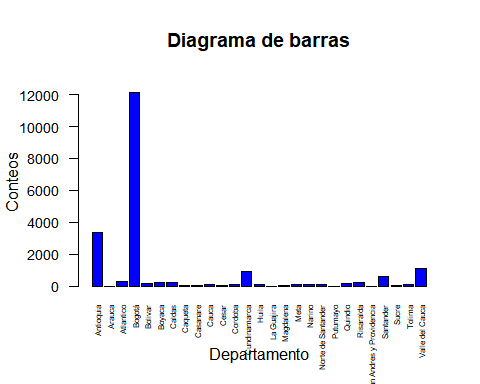
\includegraphics{Ejemplo-Regresión-Múltiple_files/figure-latex/unnamed-chunk-4-1.pdf}

\emph{\textbf{Otra forma:}}

\begin{Shaded}
\begin{Highlighting}[]
\KeywordTok{corrgram}\NormalTok{(datos, }\DataTypeTok{order=}\OtherTok{NULL}\NormalTok{, }\DataTypeTok{lower.panel=}\NormalTok{panel.shade,}
         \DataTypeTok{upper.panel=}\OtherTok{NULL}\NormalTok{, }\DataTypeTok{text.panel=}\NormalTok{panel.txt,}
         \DataTypeTok{main=}\StringTok{"Matriz de Correlaciones"}\NormalTok{)}
\end{Highlighting}
\end{Shaded}

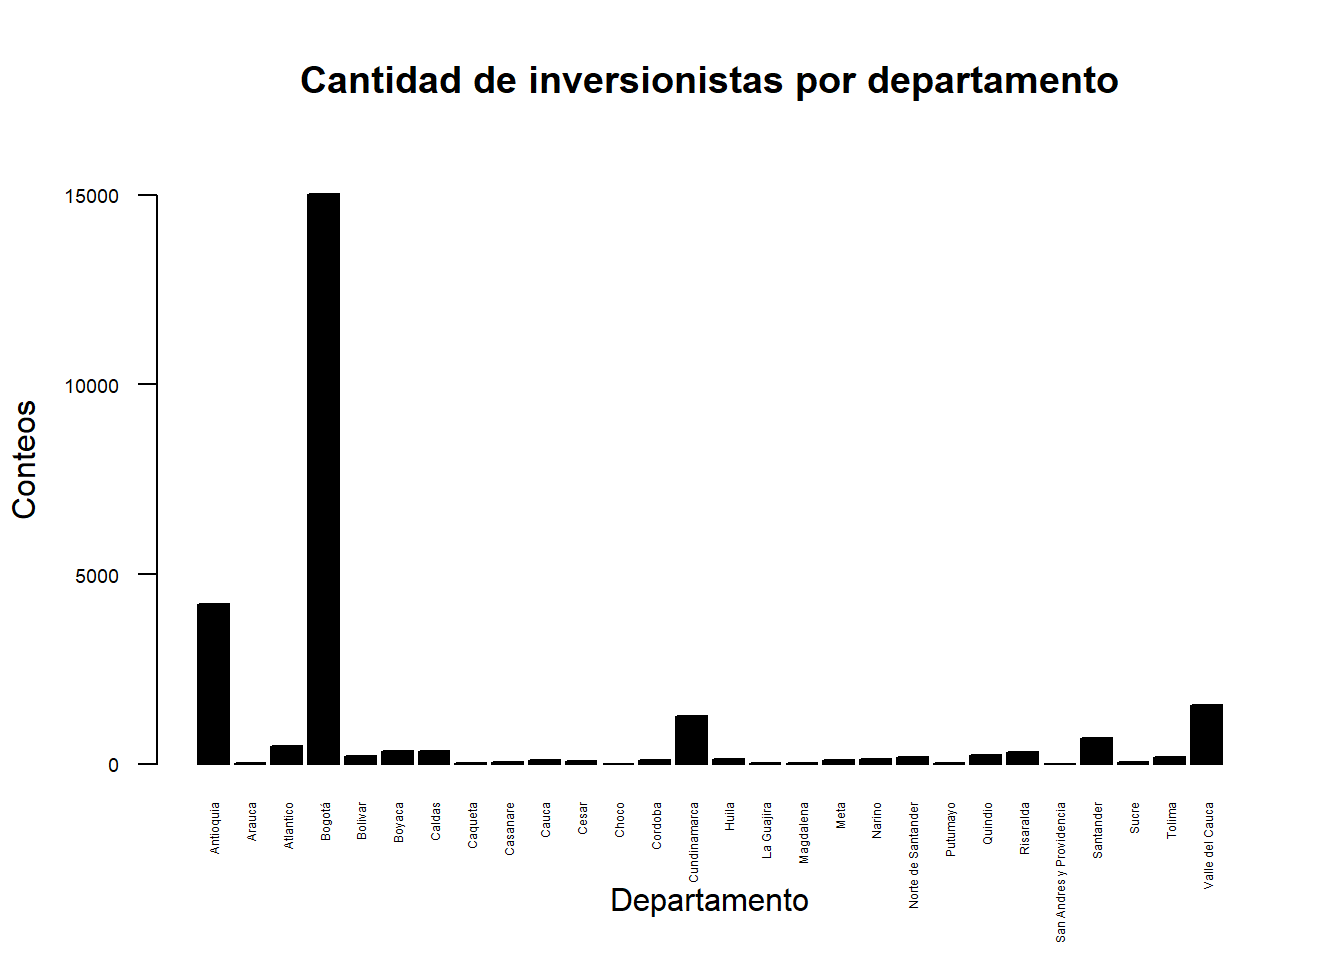
\includegraphics{Ejemplo-Regresión-Múltiple_files/figure-latex/unnamed-chunk-5-1.pdf}

\emph{\textbf{Asignando las correlaciones}}

\begin{Shaded}
\begin{Highlighting}[]
\NormalTok{mydata.cor =}\StringTok{ }\KeywordTok{cor}\NormalTok{(datos)}
\NormalTok{knitr}\OperatorTok{::}\KeywordTok{kable}\NormalTok{(}
\NormalTok{mydata.cor}
\NormalTok{)}
\end{Highlighting}
\end{Shaded}

\begin{longtable}[]{@{}lrrrrrrrrr@{}}
\toprule
\begin{minipage}[b]{0.09\columnwidth}\raggedright\strut
\strut
\end{minipage} & \begin{minipage}[b]{0.07\columnwidth}\raggedleft\strut
habitantes\strut
\end{minipage} & \begin{minipage}[b]{0.07\columnwidth}\raggedleft\strut
ingresos\strut
\end{minipage} & \begin{minipage}[b]{0.09\columnwidth}\raggedleft\strut
analfabetismo\strut
\end{minipage} & \begin{minipage}[b]{0.07\columnwidth}\raggedleft\strut
esp\_vida\strut
\end{minipage} & \begin{minipage}[b]{0.07\columnwidth}\raggedleft\strut
muerte\strut
\end{minipage} & \begin{minipage}[b]{0.07\columnwidth}\raggedleft\strut
graduados\strut
\end{minipage} & \begin{minipage}[b]{0.07\columnwidth}\raggedleft\strut
heladas\strut
\end{minipage} & \begin{minipage}[b]{0.07\columnwidth}\raggedleft\strut
area\strut
\end{minipage} & \begin{minipage}[b]{0.09\columnwidth}\raggedleft\strut
densidad\_pobl\strut
\end{minipage}\tabularnewline
\midrule
\endhead
\begin{minipage}[t]{0.09\columnwidth}\raggedright\strut
habitantes\strut
\end{minipage} & \begin{minipage}[t]{0.07\columnwidth}\raggedleft\strut
1.0000000\strut
\end{minipage} & \begin{minipage}[t]{0.07\columnwidth}\raggedleft\strut
0.2082276\strut
\end{minipage} & \begin{minipage}[t]{0.09\columnwidth}\raggedleft\strut
0.1076224\strut
\end{minipage} & \begin{minipage}[t]{0.07\columnwidth}\raggedleft\strut
-0.0680520\strut
\end{minipage} & \begin{minipage}[t]{0.07\columnwidth}\raggedleft\strut
0.3436428\strut
\end{minipage} & \begin{minipage}[t]{0.07\columnwidth}\raggedleft\strut
-0.0984897\strut
\end{minipage} & \begin{minipage}[t]{0.07\columnwidth}\raggedleft\strut
-0.3321525\strut
\end{minipage} & \begin{minipage}[t]{0.07\columnwidth}\raggedleft\strut
0.0225438\strut
\end{minipage} & \begin{minipage}[t]{0.09\columnwidth}\raggedleft\strut
0.2462279\strut
\end{minipage}\tabularnewline
\begin{minipage}[t]{0.09\columnwidth}\raggedright\strut
ingresos\strut
\end{minipage} & \begin{minipage}[t]{0.07\columnwidth}\raggedleft\strut
0.2082276\strut
\end{minipage} & \begin{minipage}[t]{0.07\columnwidth}\raggedleft\strut
1.0000000\strut
\end{minipage} & \begin{minipage}[t]{0.09\columnwidth}\raggedleft\strut
-0.4370752\strut
\end{minipage} & \begin{minipage}[t]{0.07\columnwidth}\raggedleft\strut
0.3402553\strut
\end{minipage} & \begin{minipage}[t]{0.07\columnwidth}\raggedleft\strut
-0.2300776\strut
\end{minipage} & \begin{minipage}[t]{0.07\columnwidth}\raggedleft\strut
0.6199323\strut
\end{minipage} & \begin{minipage}[t]{0.07\columnwidth}\raggedleft\strut
0.2262822\strut
\end{minipage} & \begin{minipage}[t]{0.07\columnwidth}\raggedleft\strut
0.3633154\strut
\end{minipage} & \begin{minipage}[t]{0.09\columnwidth}\raggedleft\strut
0.3299683\strut
\end{minipage}\tabularnewline
\begin{minipage}[t]{0.09\columnwidth}\raggedright\strut
analfabetismo\strut
\end{minipage} & \begin{minipage}[t]{0.07\columnwidth}\raggedleft\strut
0.1076224\strut
\end{minipage} & \begin{minipage}[t]{0.07\columnwidth}\raggedleft\strut
-0.4370752\strut
\end{minipage} & \begin{minipage}[t]{0.09\columnwidth}\raggedleft\strut
1.0000000\strut
\end{minipage} & \begin{minipage}[t]{0.07\columnwidth}\raggedleft\strut
-0.5884779\strut
\end{minipage} & \begin{minipage}[t]{0.07\columnwidth}\raggedleft\strut
0.7029752\strut
\end{minipage} & \begin{minipage}[t]{0.07\columnwidth}\raggedleft\strut
-0.6571886\strut
\end{minipage} & \begin{minipage}[t]{0.07\columnwidth}\raggedleft\strut
-0.6719470\strut
\end{minipage} & \begin{minipage}[t]{0.07\columnwidth}\raggedleft\strut
0.0772611\strut
\end{minipage} & \begin{minipage}[t]{0.09\columnwidth}\raggedleft\strut
0.0092743\strut
\end{minipage}\tabularnewline
\begin{minipage}[t]{0.09\columnwidth}\raggedright\strut
esp\_vida\strut
\end{minipage} & \begin{minipage}[t]{0.07\columnwidth}\raggedleft\strut
-0.0680520\strut
\end{minipage} & \begin{minipage}[t]{0.07\columnwidth}\raggedleft\strut
0.3402553\strut
\end{minipage} & \begin{minipage}[t]{0.09\columnwidth}\raggedleft\strut
-0.5884779\strut
\end{minipage} & \begin{minipage}[t]{0.07\columnwidth}\raggedleft\strut
1.0000000\strut
\end{minipage} & \begin{minipage}[t]{0.07\columnwidth}\raggedleft\strut
-0.7808458\strut
\end{minipage} & \begin{minipage}[t]{0.07\columnwidth}\raggedleft\strut
0.5822162\strut
\end{minipage} & \begin{minipage}[t]{0.07\columnwidth}\raggedleft\strut
0.2620680\strut
\end{minipage} & \begin{minipage}[t]{0.07\columnwidth}\raggedleft\strut
-0.1073319\strut
\end{minipage} & \begin{minipage}[t]{0.09\columnwidth}\raggedleft\strut
0.0910618\strut
\end{minipage}\tabularnewline
\begin{minipage}[t]{0.09\columnwidth}\raggedright\strut
muerte\strut
\end{minipage} & \begin{minipage}[t]{0.07\columnwidth}\raggedleft\strut
0.3436428\strut
\end{minipage} & \begin{minipage}[t]{0.07\columnwidth}\raggedleft\strut
-0.2300776\strut
\end{minipage} & \begin{minipage}[t]{0.09\columnwidth}\raggedleft\strut
0.7029752\strut
\end{minipage} & \begin{minipage}[t]{0.07\columnwidth}\raggedleft\strut
-0.7808458\strut
\end{minipage} & \begin{minipage}[t]{0.07\columnwidth}\raggedleft\strut
1.0000000\strut
\end{minipage} & \begin{minipage}[t]{0.07\columnwidth}\raggedleft\strut
-0.4879710\strut
\end{minipage} & \begin{minipage}[t]{0.07\columnwidth}\raggedleft\strut
-0.5388834\strut
\end{minipage} & \begin{minipage}[t]{0.07\columnwidth}\raggedleft\strut
0.2283902\strut
\end{minipage} & \begin{minipage}[t]{0.09\columnwidth}\raggedleft\strut
-0.1850352\strut
\end{minipage}\tabularnewline
\begin{minipage}[t]{0.09\columnwidth}\raggedright\strut
graduados\strut
\end{minipage} & \begin{minipage}[t]{0.07\columnwidth}\raggedleft\strut
-0.0984897\strut
\end{minipage} & \begin{minipage}[t]{0.07\columnwidth}\raggedleft\strut
0.6199323\strut
\end{minipage} & \begin{minipage}[t]{0.09\columnwidth}\raggedleft\strut
-0.6571886\strut
\end{minipage} & \begin{minipage}[t]{0.07\columnwidth}\raggedleft\strut
0.5822162\strut
\end{minipage} & \begin{minipage}[t]{0.07\columnwidth}\raggedleft\strut
-0.4879710\strut
\end{minipage} & \begin{minipage}[t]{0.07\columnwidth}\raggedleft\strut
1.0000000\strut
\end{minipage} & \begin{minipage}[t]{0.07\columnwidth}\raggedleft\strut
0.3667797\strut
\end{minipage} & \begin{minipage}[t]{0.07\columnwidth}\raggedleft\strut
0.3335419\strut
\end{minipage} & \begin{minipage}[t]{0.09\columnwidth}\raggedleft\strut
-0.0883672\strut
\end{minipage}\tabularnewline
\begin{minipage}[t]{0.09\columnwidth}\raggedright\strut
heladas\strut
\end{minipage} & \begin{minipage}[t]{0.07\columnwidth}\raggedleft\strut
-0.3321525\strut
\end{minipage} & \begin{minipage}[t]{0.07\columnwidth}\raggedleft\strut
0.2262822\strut
\end{minipage} & \begin{minipage}[t]{0.09\columnwidth}\raggedleft\strut
-0.6719470\strut
\end{minipage} & \begin{minipage}[t]{0.07\columnwidth}\raggedleft\strut
0.2620680\strut
\end{minipage} & \begin{minipage}[t]{0.07\columnwidth}\raggedleft\strut
-0.5388834\strut
\end{minipage} & \begin{minipage}[t]{0.07\columnwidth}\raggedleft\strut
0.3667797\strut
\end{minipage} & \begin{minipage}[t]{0.07\columnwidth}\raggedleft\strut
1.0000000\strut
\end{minipage} & \begin{minipage}[t]{0.07\columnwidth}\raggedleft\strut
0.0592291\strut
\end{minipage} & \begin{minipage}[t]{0.09\columnwidth}\raggedleft\strut
0.0022767\strut
\end{minipage}\tabularnewline
\begin{minipage}[t]{0.09\columnwidth}\raggedright\strut
area\strut
\end{minipage} & \begin{minipage}[t]{0.07\columnwidth}\raggedleft\strut
0.0225438\strut
\end{minipage} & \begin{minipage}[t]{0.07\columnwidth}\raggedleft\strut
0.3633154\strut
\end{minipage} & \begin{minipage}[t]{0.09\columnwidth}\raggedleft\strut
0.0772611\strut
\end{minipage} & \begin{minipage}[t]{0.07\columnwidth}\raggedleft\strut
-0.1073319\strut
\end{minipage} & \begin{minipage}[t]{0.07\columnwidth}\raggedleft\strut
0.2283902\strut
\end{minipage} & \begin{minipage}[t]{0.07\columnwidth}\raggedleft\strut
0.3335419\strut
\end{minipage} & \begin{minipage}[t]{0.07\columnwidth}\raggedleft\strut
0.0592291\strut
\end{minipage} & \begin{minipage}[t]{0.07\columnwidth}\raggedleft\strut
1.0000000\strut
\end{minipage} & \begin{minipage}[t]{0.09\columnwidth}\raggedleft\strut
-0.3413885\strut
\end{minipage}\tabularnewline
\begin{minipage}[t]{0.09\columnwidth}\raggedright\strut
densidad\_pobl\strut
\end{minipage} & \begin{minipage}[t]{0.07\columnwidth}\raggedleft\strut
0.2462279\strut
\end{minipage} & \begin{minipage}[t]{0.07\columnwidth}\raggedleft\strut
0.3299683\strut
\end{minipage} & \begin{minipage}[t]{0.09\columnwidth}\raggedleft\strut
0.0092743\strut
\end{minipage} & \begin{minipage}[t]{0.07\columnwidth}\raggedleft\strut
0.0910618\strut
\end{minipage} & \begin{minipage}[t]{0.07\columnwidth}\raggedleft\strut
-0.1850352\strut
\end{minipage} & \begin{minipage}[t]{0.07\columnwidth}\raggedleft\strut
-0.0883672\strut
\end{minipage} & \begin{minipage}[t]{0.07\columnwidth}\raggedleft\strut
0.0022767\strut
\end{minipage} & \begin{minipage}[t]{0.07\columnwidth}\raggedleft\strut
-0.3413885\strut
\end{minipage} & \begin{minipage}[t]{0.09\columnwidth}\raggedleft\strut
1.0000000\strut
\end{minipage}\tabularnewline
\bottomrule
\end{longtable}

\begin{Shaded}
\begin{Highlighting}[]
\CommentTok{# install.packages("corrplot")}
\KeywordTok{library}\NormalTok{(corrplot)}
\end{Highlighting}
\end{Shaded}

\begin{verbatim}
## corrplot 0.88 loaded
\end{verbatim}

\begin{Shaded}
\begin{Highlighting}[]
\KeywordTok{corrplot}\NormalTok{(mydata.cor)}
\end{Highlighting}
\end{Shaded}

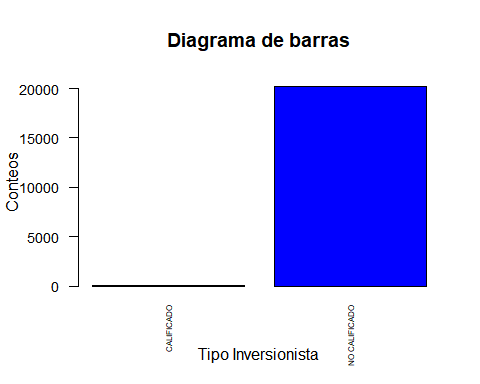
\includegraphics{Ejemplo-Regresión-Múltiple_files/figure-latex/unnamed-chunk-6-1.pdf}

\begin{Shaded}
\begin{Highlighting}[]
\KeywordTok{corrplot}\NormalTok{(mydata.cor, }\DataTypeTok{type =} \StringTok{"upper"}\NormalTok{, }\DataTypeTok{order =} \StringTok{"hclust"}\NormalTok{, }\DataTypeTok{tl.col =} \StringTok{"black"}\NormalTok{, }\DataTypeTok{tl.srt =} \DecValTok{45}\NormalTok{)}
\end{Highlighting}
\end{Shaded}

\includegraphics{Ejemplo-Regresión-Múltiple_files/figure-latex/unnamed-chunk-6-2.pdf}

\begin{Shaded}
\begin{Highlighting}[]
\KeywordTok{corrplot}\NormalTok{(mydata.cor, }\DataTypeTok{type =} \StringTok{"lower"}\NormalTok{, }\DataTypeTok{order =} \StringTok{"hclust"}\NormalTok{, }\DataTypeTok{tl.col =} \StringTok{"black"}\NormalTok{, }\DataTypeTok{tl.srt =} \DecValTok{45}\NormalTok{)}
\end{Highlighting}
\end{Shaded}

\includegraphics{Ejemplo-Regresión-Múltiple_files/figure-latex/unnamed-chunk-6-3.pdf}

\emph{\textbf{Ahora supervisamos el comportamiento distribucional de las
variables:}}

\begin{Shaded}
\begin{Highlighting}[]
\KeywordTok{library}\NormalTok{(psych)}
\KeywordTok{multi.hist}\NormalTok{(}\DataTypeTok{x =}\NormalTok{ mydata.cor, }\DataTypeTok{dcol =} \KeywordTok{c}\NormalTok{(}\StringTok{"blue"}\NormalTok{, }\StringTok{"red"}\NormalTok{), }\DataTypeTok{dlty =} \KeywordTok{c}\NormalTok{(}\StringTok{"dotted"}\NormalTok{, }\StringTok{"solid"}\NormalTok{))}
\end{Highlighting}
\end{Shaded}

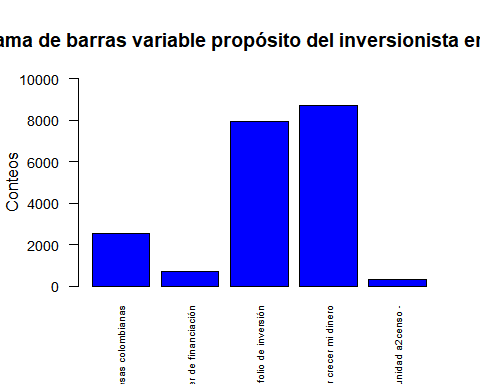
\includegraphics{Ejemplo-Regresión-Múltiple_files/figure-latex/unnamed-chunk-7-1.pdf}

\emph{\textbf{Combinando histogramas con Regresiones y Correlaciones:}}

\begin{Shaded}
\begin{Highlighting}[]
\KeywordTok{library}\NormalTok{(GGally)}
\KeywordTok{ggpairs}\NormalTok{(datos, }\DataTypeTok{lower =} \KeywordTok{list}\NormalTok{(}\DataTypeTok{continuous =} \StringTok{"smooth"}\NormalTok{),}\DataTypeTok{diag =} \KeywordTok{list}\NormalTok{(}\DataTypeTok{continuous =} \StringTok{"bar"}\NormalTok{), }\DataTypeTok{axisLabels =} \StringTok{"none"}\NormalTok{)}
\end{Highlighting}
\end{Shaded}

\begin{verbatim}
## Warning in check_and_set_ggpairs_defaults("diag", diag, continuous =
## "densityDiag", : Changing diag$continuous from 'bar' to 'barDiag'
\end{verbatim}

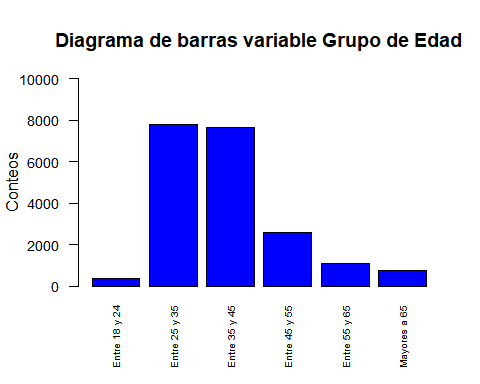
\includegraphics{Ejemplo-Regresión-Múltiple_files/figure-latex/unnamed-chunk-8-1.pdf}

\subsubsection{MODELO DE REGRESIÓN LINEAL
MÚLTIPLE:}\label{modelo-de-regresiuxf3n-lineal-muxfaltiple}

\emph{\textbf{2. Generar el modelo:}}

\begin{Shaded}
\begin{Highlighting}[]
\NormalTok{modelo <-}\StringTok{ }\KeywordTok{lm}\NormalTok{(esp_vida }\OperatorTok{~}\StringTok{ }\NormalTok{habitantes }\OperatorTok{+}\StringTok{ }\NormalTok{ingresos }\OperatorTok{+}\StringTok{ }\NormalTok{analfabetismo }\OperatorTok{+}\StringTok{ }\NormalTok{muerte }\OperatorTok{+}\StringTok{ }\NormalTok{graduados }\OperatorTok{+}\StringTok{ }\NormalTok{heladas }\OperatorTok{+}\StringTok{ }\NormalTok{area }\OperatorTok{+}\StringTok{ }\NormalTok{densidad_pobl, }\DataTypeTok{data =}\NormalTok{ datos )}

\KeywordTok{summary}\NormalTok{(modelo)}
\end{Highlighting}
\end{Shaded}

\begin{verbatim}
## 
## Call:
## lm(formula = esp_vida ~ habitantes + ingresos + analfabetismo + 
##     muerte + graduados + heladas + area + densidad_pobl, data = datos)
## 
## Residuals:
##      Min       1Q   Median       3Q      Max 
## -1.47514 -0.45887 -0.06352  0.59362  1.21823 
## 
## Coefficients:
##                 Estimate Std. Error t value Pr(>|t|)    
## (Intercept)    6.995e+01  1.843e+00  37.956  < 2e-16 ***
## habitantes     6.480e-05  3.001e-05   2.159   0.0367 *  
## ingresos       2.701e-04  3.087e-04   0.875   0.3867    
## analfabetismo  3.029e-01  4.024e-01   0.753   0.4559    
## muerte        -3.286e-01  4.941e-02  -6.652 5.12e-08 ***
## graduados      4.291e-02  2.332e-02   1.840   0.0730 .  
## heladas       -4.580e-03  3.189e-03  -1.436   0.1585    
## area          -1.558e-06  1.914e-06  -0.814   0.4205    
## densidad_pobl -1.105e-03  7.312e-04  -1.511   0.1385    
## ---
## Signif. codes:  0 '***' 0.001 '**' 0.01 '*' 0.05 '.' 0.1 ' ' 1
## 
## Residual standard error: 0.7337 on 41 degrees of freedom
## Multiple R-squared:  0.7501, Adjusted R-squared:  0.7013 
## F-statistic: 15.38 on 8 and 41 DF,  p-value: 3.787e-10
\end{verbatim}

\emph{\textbf{Predicciones de Y}}

\begin{Shaded}
\begin{Highlighting}[]
\NormalTok{Predicciones<-modelo}\OperatorTok{$}\NormalTok{fitted.values}
\CommentTok{# Predicciones}

\NormalTok{Y_dataset=datos}\OperatorTok{$}\NormalTok{esp_vida}
\NormalTok{Y_modelad=Predicciones}
\NormalTok{Comparativo=}\KeywordTok{cbind}\NormalTok{(Y_dataset, Y_modelad)}
\NormalTok{Comparativo}
\end{Highlighting}
\end{Shaded}

\begin{verbatim}
##                Y_dataset Y_modelad
## Alabama            69.05  68.35977
## Alaska             69.31  69.70301
## Arizona            70.55  71.52509
## Arkansas           70.66  69.54425
## California         71.71  71.85457
## Colorado           72.06  71.20429
## Connecticut        72.48  71.96438
## Delaware           70.06  71.06704
## Florida            70.66  70.61781
## Georgia            68.54  68.69550
## Hawaii             73.60  72.38177
## Idaho              71.87  71.39185
## Illinois           70.14  70.30948
## Indiana            70.88  70.86968
## Iowa               72.56  72.52812
## Kansas             72.58  71.95195
## Kentucky           70.10  69.23420
## Louisiana          68.76  69.25668
## Maine              70.39  71.86514
## Maryland           70.22  70.43356
## Massachusetts      71.83  72.06557
## Michigan           70.63  69.87605
## Minnesota          72.96  72.45362
## Mississippi        68.09  68.95961
## Missouri           70.69  70.00970
## Montana            70.56  71.30919
## Nebraska           72.60  72.26312
## Nevada             69.03  69.51082
## New Hampshire      71.23  71.84796
## New Jersey         70.93  71.10140
## New Mexico         70.32  70.09502
## New York           70.55  70.68151
## North Carolina     69.21  69.33322
## North Dakota       72.78  72.33620
## Ohio               70.82  71.04983
## Oklahoma           71.42  71.11975
## Oregon             72.13  72.35542
## Pennsylvania       70.43  71.43424
## Rhode Island       71.90  71.27399
## South Carolina     67.96  69.17325
## South Dakota       72.08  72.08382
## Tennessee          70.11  69.44971
## Texas              70.90  69.94504
## Utah               72.90  71.93372
## Vermont            71.64  71.02037
## Virginia           70.08  70.30622
## Washington         71.72  72.67871
## West Virginia      69.48  70.47298
## Wisconsin          72.48  72.15882
## Wyoming            70.29  70.87300
\end{verbatim}

\begin{Shaded}
\begin{Highlighting}[]
\NormalTok{Diferecias=Y_dataset}\OperatorTok{-}\NormalTok{Y_modelad}
\NormalTok{Errores=}\KeywordTok{cbind}\NormalTok{(Comparativo, Diferecias)}
\NormalTok{Errores}
\end{Highlighting}
\end{Shaded}

\begin{verbatim}
##                Y_dataset Y_modelad   Diferecias
## Alabama            69.05  68.35977  0.690233077
## Alaska             69.31  69.70301 -0.393014184
## Arizona            70.55  71.52509 -0.975085207
## Arkansas           70.66  69.54425  1.115751828
## California         71.71  71.85457 -0.144571583
## Colorado           72.06  71.20429  0.855706129
## Connecticut        72.48  71.96438  0.515615350
## Delaware           70.06  71.06704 -1.007038925
## Florida            70.66  70.61781  0.042194324
## Georgia            68.54  68.69550 -0.155498340
## Hawaii             73.60  72.38177  1.218230800
## Idaho              71.87  71.39185  0.478147392
## Illinois           70.14  70.30948 -0.169478852
## Indiana            70.88  70.86968  0.010319513
## Iowa               72.56  72.52812  0.031875031
## Kansas             72.58  71.95195  0.628047720
## Kentucky           70.10  69.23420  0.865798949
## Louisiana          68.76  69.25668 -0.496676230
## Maine              70.39  71.86514 -1.475141857
## Maryland           70.22  70.43356 -0.213558902
## Massachusetts      71.83  72.06557 -0.235568739
## Michigan           70.63  69.87605  0.753949012
## Minnesota          72.96  72.45362  0.506382389
## Mississippi        68.09  68.95961 -0.869608746
## Missouri           70.69  70.00970  0.680303836
## Montana            70.56  71.30919 -0.749187924
## Nebraska           72.60  72.26312  0.336878262
## Nevada             69.03  69.51082 -0.480816117
## New Hampshire      71.23  71.84796 -0.617962700
## New Jersey         70.93  71.10140 -0.171398845
## New Mexico         70.32  70.09502  0.224976927
## New York           70.55  70.68151 -0.131513872
## North Carolina     69.21  69.33322 -0.123216068
## North Dakota       72.78  72.33620  0.443800848
## Ohio               70.82  71.04983 -0.229827334
## Oklahoma           71.42  71.11975  0.300248058
## Oregon             72.13  72.35542 -0.225416625
## Pennsylvania       70.43  71.43424 -1.004244727
## Rhode Island       71.90  71.27399  0.626013701
## South Carolina     67.96  69.17325 -1.213253410
## South Dakota       72.08  72.08382 -0.003822235
## Tennessee          70.11  69.44971  0.660293306
## Texas              70.90  69.94504  0.954955228
## Utah               72.90  71.93372  0.966275651
## Vermont            71.64  71.02037  0.619627679
## Virginia           70.08  70.30622 -0.226217258
## Washington         71.72  72.67871 -0.958709507
## West Virginia      69.48  70.47298 -0.992977983
## Wisconsin          72.48  72.15882  0.321179837
## Wyoming            70.29  70.87300 -0.582998678
\end{verbatim}

\begin{Shaded}
\begin{Highlighting}[]
\CommentTok{# Según el supuesto de Mínimos Cuadrados}
\CommentTok{# La suma (promedio) de los Errores ~ 0:}
\NormalTok{SupuestErrores=}\KeywordTok{mean}\NormalTok{(Errores[,}\DecValTok{3}\NormalTok{])}
\NormalTok{SupuestErrores}
\end{Highlighting}
\end{Shaded}

\begin{verbatim}
## [1] 2.84203e-16
\end{verbatim}

\emph{\textbf{Que ocurre si eliminamos alguna de las variables
predictoras?, Corramos el modelo únicamente con las variables
significativas del ajuste inicial}}

\begin{Shaded}
\begin{Highlighting}[]
\NormalTok{modelo <-}\StringTok{ }\KeywordTok{lm}\NormalTok{(esp_vida }\OperatorTok{~}\StringTok{ }\NormalTok{habitantes }\OperatorTok{+}\StringTok{  }\NormalTok{muerte, }\DataTypeTok{data =}\NormalTok{ datos )}
\KeywordTok{summary}\NormalTok{(modelo)}
\end{Highlighting}
\end{Shaded}

\begin{verbatim}
## 
## Call:
## lm(formula = esp_vida ~ habitantes + muerte, data = datos)
## 
## Residuals:
##      Min       1Q   Median       3Q      Max 
## -1.73194 -0.40907 -0.06544  0.48865  2.58417 
## 
## Coefficients:
##               Estimate Std. Error t value Pr(>|t|)    
## (Intercept)  7.289e+01  2.585e-01 282.012  < 2e-16 ***
## habitantes   6.828e-05  2.742e-05   2.490   0.0164 *  
## muerte      -3.123e-01  3.317e-02  -9.417 2.15e-12 ***
## ---
## Signif. codes:  0 '***' 0.001 '**' 0.01 '*' 0.05 '.' 0.1 ' ' 1
## 
## Residual standard error: 0.8048 on 47 degrees of freedom
## Multiple R-squared:  0.6552, Adjusted R-squared:  0.6405 
## F-statistic: 44.66 on 2 and 47 DF,  p-value: 1.357e-11
\end{verbatim}

\emph{\textbf{Diagnóstico del Modelo del Modelo Inicial (Modelo con
todas las variables predictoras):}}

\begin{Shaded}
\begin{Highlighting}[]
\NormalTok{modelo <-}\StringTok{ }\KeywordTok{lm}\NormalTok{(esp_vida }\OperatorTok{~}\StringTok{ }\NormalTok{habitantes }\OperatorTok{+}\StringTok{ }\NormalTok{ingresos }\OperatorTok{+}\StringTok{ }\NormalTok{analfabetismo }\OperatorTok{+}\StringTok{ }\NormalTok{muerte }\OperatorTok{+}\StringTok{ }\NormalTok{graduados }\OperatorTok{+}\StringTok{ }\NormalTok{heladas }\OperatorTok{+}\StringTok{ }\NormalTok{area }\OperatorTok{+}\StringTok{ }\NormalTok{densidad_pobl, }\DataTypeTok{data =}\NormalTok{ datos )}


\CommentTok{# Coeficientes del Modelo (bettas)}
\KeywordTok{coefficients}\NormalTok{(modelo) }
\end{Highlighting}
\end{Shaded}

\begin{verbatim}
##   (Intercept)    habitantes      ingresos analfabetismo        muerte 
##  6.995061e+01  6.480191e-05  2.700719e-04  3.028607e-01 -3.286480e-01 
##     graduados       heladas          area densidad_pobl 
##  4.290767e-02 -4.580195e-03 -1.557759e-06 -1.104781e-03
\end{verbatim}

\begin{Shaded}
\begin{Highlighting}[]
\CommentTok{# I.C. de la estimación de los bettas}
\KeywordTok{confint}\NormalTok{(modelo, }\DataTypeTok{level=}\FloatTok{0.95}\NormalTok{) }
\end{Highlighting}
\end{Shaded}

\begin{verbatim}
##                       2.5 %        97.5 %
## (Intercept)    6.622872e+01  7.367251e+01
## habitantes     4.192906e-06  1.254109e-04
## ingresos      -3.533399e-04  8.934837e-04
## analfabetismo -5.097129e-01  1.115434e+00
## muerte        -4.284249e-01 -2.288711e-01
## graduados     -4.184247e-03  8.999959e-02
## heladas       -1.102098e-02  1.860585e-03
## area          -5.423922e-06  2.308404e-06
## densidad_pobl -2.581440e-03  3.718781e-04
\end{verbatim}

\begin{Shaded}
\begin{Highlighting}[]
\CommentTok{# Predicciones}
\KeywordTok{fitted}\NormalTok{(modelo) }
\end{Highlighting}
\end{Shaded}

\begin{verbatim}
##        Alabama         Alaska        Arizona       Arkansas     California 
##       68.35977       69.70301       71.52509       69.54425       71.85457 
##       Colorado    Connecticut       Delaware        Florida        Georgia 
##       71.20429       71.96438       71.06704       70.61781       68.69550 
##         Hawaii          Idaho       Illinois        Indiana           Iowa 
##       72.38177       71.39185       70.30948       70.86968       72.52812 
##         Kansas       Kentucky      Louisiana          Maine       Maryland 
##       71.95195       69.23420       69.25668       71.86514       70.43356 
##  Massachusetts       Michigan      Minnesota    Mississippi       Missouri 
##       72.06557       69.87605       72.45362       68.95961       70.00970 
##        Montana       Nebraska         Nevada  New Hampshire     New Jersey 
##       71.30919       72.26312       69.51082       71.84796       71.10140 
##     New Mexico       New York North Carolina   North Dakota           Ohio 
##       70.09502       70.68151       69.33322       72.33620       71.04983 
##       Oklahoma         Oregon   Pennsylvania   Rhode Island South Carolina 
##       71.11975       72.35542       71.43424       71.27399       69.17325 
##   South Dakota      Tennessee          Texas           Utah        Vermont 
##       72.08382       69.44971       69.94504       71.93372       71.02037 
##       Virginia     Washington  West Virginia      Wisconsin        Wyoming 
##       70.30622       72.67871       70.47298       72.15882       70.87300
\end{verbatim}

\begin{Shaded}
\begin{Highlighting}[]
\CommentTok{# residuales}
\KeywordTok{residuals}\NormalTok{(modelo) }
\end{Highlighting}
\end{Shaded}

\begin{verbatim}
##        Alabama         Alaska        Arizona       Arkansas     California 
##    0.690233077   -0.393014184   -0.975085207    1.115751828   -0.144571583 
##       Colorado    Connecticut       Delaware        Florida        Georgia 
##    0.855706129    0.515615350   -1.007038925    0.042194324   -0.155498340 
##         Hawaii          Idaho       Illinois        Indiana           Iowa 
##    1.218230800    0.478147392   -0.169478852    0.010319513    0.031875031 
##         Kansas       Kentucky      Louisiana          Maine       Maryland 
##    0.628047720    0.865798949   -0.496676230   -1.475141857   -0.213558902 
##  Massachusetts       Michigan      Minnesota    Mississippi       Missouri 
##   -0.235568739    0.753949012    0.506382389   -0.869608746    0.680303836 
##        Montana       Nebraska         Nevada  New Hampshire     New Jersey 
##   -0.749187924    0.336878262   -0.480816117   -0.617962700   -0.171398845 
##     New Mexico       New York North Carolina   North Dakota           Ohio 
##    0.224976927   -0.131513872   -0.123216068    0.443800848   -0.229827334 
##       Oklahoma         Oregon   Pennsylvania   Rhode Island South Carolina 
##    0.300248058   -0.225416625   -1.004244727    0.626013701   -1.213253410 
##   South Dakota      Tennessee          Texas           Utah        Vermont 
##   -0.003822235    0.660293306    0.954955228    0.966275651    0.619627679 
##       Virginia     Washington  West Virginia      Wisconsin        Wyoming 
##   -0.226217258   -0.958709507   -0.992977983    0.321179837   -0.582998678
\end{verbatim}

\begin{Shaded}
\begin{Highlighting}[]
\CommentTok{# Tabla ANOVA}
\NormalTok{knitr}\OperatorTok{::}\KeywordTok{kable}\NormalTok{(}
\KeywordTok{anova}\NormalTok{(modelo) }
\NormalTok{)}
\end{Highlighting}
\end{Shaded}

\begin{longtable}[]{@{}lrrrrr@{}}
\toprule
& Df & Sum Sq & Mean Sq & F value & Pr(\textgreater{}F)\tabularnewline
\midrule
\endhead
habitantes & 1 & 0.4089187 & 0.4089187 & 0.7597160 &
0.3884929\tabularnewline
ingresos & 1 & 11.5946306 & 11.5946306 & 21.5412666 &
0.0000353\tabularnewline
analfabetismo & 1 & 19.4207309 & 19.4207309 & 36.0811100 &
0.0000004\tabularnewline
muerte & 1 & 27.4288381 & 27.4288381 & 50.9590976 &
0.0000000\tabularnewline
graduados & 1 & 4.0988911 & 4.0988911 & 7.6151892 &
0.0086125\tabularnewline
heladas & 1 & 2.0487679 & 2.0487679 & 3.8063356 &
0.0579156\tabularnewline
area & 1 & 0.0010866 & 0.0010866 & 0.0020187 & 0.9643811\tabularnewline
densidad\_pobl & 1 & 1.2288046 & 1.2288046 & 2.2829540 &
0.1384722\tabularnewline
Residuals & 41 & 22.0683335 & 0.5382520 & NA & NA\tabularnewline
\bottomrule
\end{longtable}

\begin{Shaded}
\begin{Highlighting}[]
\CommentTok{# La Matriz de Covarianzas del Modelo}
\NormalTok{knitr}\OperatorTok{::}\KeywordTok{kable}\NormalTok{(}
\KeywordTok{vcov}\NormalTok{(modelo) }
\NormalTok{)}
\end{Highlighting}
\end{Shaded}

\begin{longtable}[]{@{}lrrrrrrrrr@{}}
\toprule
\begin{minipage}[b]{0.09\columnwidth}\raggedright\strut
\strut
\end{minipage} & \begin{minipage}[b]{0.07\columnwidth}\raggedleft\strut
(Intercept)\strut
\end{minipage} & \begin{minipage}[b]{0.07\columnwidth}\raggedleft\strut
habitantes\strut
\end{minipage} & \begin{minipage}[b]{0.07\columnwidth}\raggedleft\strut
ingresos\strut
\end{minipage} & \begin{minipage}[b]{0.09\columnwidth}\raggedleft\strut
analfabetismo\strut
\end{minipage} & \begin{minipage}[b]{0.07\columnwidth}\raggedleft\strut
muerte\strut
\end{minipage} & \begin{minipage}[b]{0.07\columnwidth}\raggedleft\strut
graduados\strut
\end{minipage} & \begin{minipage}[b]{0.07\columnwidth}\raggedleft\strut
heladas\strut
\end{minipage} & \begin{minipage}[b]{0.06\columnwidth}\raggedleft\strut
area\strut
\end{minipage} & \begin{minipage}[b]{0.09\columnwidth}\raggedleft\strut
densidad\_pobl\strut
\end{minipage}\tabularnewline
\midrule
\endhead
\begin{minipage}[t]{0.09\columnwidth}\raggedright\strut
(Intercept)\strut
\end{minipage} & \begin{minipage}[t]{0.07\columnwidth}\raggedleft\strut
3.3964314\strut
\end{minipage} & \begin{minipage}[t]{0.07\columnwidth}\raggedleft\strut
-8.5e-06\strut
\end{minipage} & \begin{minipage}[t]{0.07\columnwidth}\raggedleft\strut
-0.0002757\strut
\end{minipage} & \begin{minipage}[t]{0.09\columnwidth}\raggedleft\strut
-0.5507936\strut
\end{minipage} & \begin{minipage}[t]{0.07\columnwidth}\raggedleft\strut
-0.0081216\strut
\end{minipage} & \begin{minipage}[t]{0.07\columnwidth}\raggedleft\strut
-0.0245238\strut
\end{minipage} & \begin{minipage}[t]{0.07\columnwidth}\raggedleft\strut
-0.0034130\strut
\end{minipage} & \begin{minipage}[t]{0.06\columnwidth}\raggedleft\strut
2.3e-06\strut
\end{minipage} & \begin{minipage}[t]{0.09\columnwidth}\raggedleft\strut
0.0004804\strut
\end{minipage}\tabularnewline
\begin{minipage}[t]{0.09\columnwidth}\raggedright\strut
habitantes\strut
\end{minipage} & \begin{minipage}[t]{0.07\columnwidth}\raggedleft\strut
-0.0000085\strut
\end{minipage} & \begin{minipage}[t]{0.07\columnwidth}\raggedleft\strut
0.0e+00\strut
\end{minipage} & \begin{minipage}[t]{0.07\columnwidth}\raggedleft\strut
0.0000000\strut
\end{minipage} & \begin{minipage}[t]{0.09\columnwidth}\raggedleft\strut
0.0000043\strut
\end{minipage} & \begin{minipage}[t]{0.07\columnwidth}\raggedleft\strut
-0.0000006\strut
\end{minipage} & \begin{minipage}[t]{0.07\columnwidth}\raggedleft\strut
0.0000001\strut
\end{minipage} & \begin{minipage}[t]{0.07\columnwidth}\raggedleft\strut
0.0000000\strut
\end{minipage} & \begin{minipage}[t]{0.06\columnwidth}\raggedleft\strut
0.0e+00\strut
\end{minipage} & \begin{minipage}[t]{0.09\columnwidth}\raggedleft\strut
0.0000000\strut
\end{minipage}\tabularnewline
\begin{minipage}[t]{0.09\columnwidth}\raggedright\strut
ingresos\strut
\end{minipage} & \begin{minipage}[t]{0.07\columnwidth}\raggedleft\strut
-0.0002757\strut
\end{minipage} & \begin{minipage}[t]{0.07\columnwidth}\raggedleft\strut
0.0e+00\strut
\end{minipage} & \begin{minipage}[t]{0.07\columnwidth}\raggedleft\strut
0.0000001\strut
\end{minipage} & \begin{minipage}[t]{0.09\columnwidth}\raggedleft\strut
0.0000427\strut
\end{minipage} & \begin{minipage}[t]{0.07\columnwidth}\raggedleft\strut
-0.0000030\strut
\end{minipage} & \begin{minipage}[t]{0.07\columnwidth}\raggedleft\strut
-0.0000027\strut
\end{minipage} & \begin{minipage}[t]{0.07\columnwidth}\raggedleft\strut
0.0000001\strut
\end{minipage} & \begin{minipage}[t]{0.06\columnwidth}\raggedleft\strut
0.0e+00\strut
\end{minipage} & \begin{minipage}[t]{0.09\columnwidth}\raggedleft\strut
-0.0000001\strut
\end{minipage}\tabularnewline
\begin{minipage}[t]{0.09\columnwidth}\raggedright\strut
analfabetismo\strut
\end{minipage} & \begin{minipage}[t]{0.07\columnwidth}\raggedleft\strut
-0.5507936\strut
\end{minipage} & \begin{minipage}[t]{0.07\columnwidth}\raggedleft\strut
4.3e-06\strut
\end{minipage} & \begin{minipage}[t]{0.07\columnwidth}\raggedleft\strut
0.0000427\strut
\end{minipage} & \begin{minipage}[t]{0.09\columnwidth}\raggedleft\strut
0.1618900\strut
\end{minipage} & \begin{minipage}[t]{0.07\columnwidth}\raggedleft\strut
-0.0087810\strut
\end{minipage} & \begin{minipage}[t]{0.07\columnwidth}\raggedleft\strut
0.0034149\strut
\end{minipage} & \begin{minipage}[t]{0.07\columnwidth}\raggedleft\strut
0.0007907\strut
\end{minipage} & \begin{minipage}[t]{0.06\columnwidth}\raggedleft\strut
-4.0e-07\strut
\end{minipage} & \begin{minipage}[t]{0.09\columnwidth}\raggedleft\strut
-0.0001302\strut
\end{minipage}\tabularnewline
\begin{minipage}[t]{0.09\columnwidth}\raggedright\strut
muerte\strut
\end{minipage} & \begin{minipage}[t]{0.07\columnwidth}\raggedleft\strut
-0.0081216\strut
\end{minipage} & \begin{minipage}[t]{0.07\columnwidth}\raggedleft\strut
-6.0e-07\strut
\end{minipage} & \begin{minipage}[t]{0.07\columnwidth}\raggedleft\strut
-0.0000030\strut
\end{minipage} & \begin{minipage}[t]{0.09\columnwidth}\raggedleft\strut
-0.0087810\strut
\end{minipage} & \begin{minipage}[t]{0.07\columnwidth}\raggedleft\strut
0.0024409\strut
\end{minipage} & \begin{minipage}[t]{0.07\columnwidth}\raggedleft\strut
0.0002771\strut
\end{minipage} & \begin{minipage}[t]{0.07\columnwidth}\raggedleft\strut
0.0000003\strut
\end{minipage} & \begin{minipage}[t]{0.06\columnwidth}\raggedleft\strut
0.0e+00\strut
\end{minipage} & \begin{minipage}[t]{0.09\columnwidth}\raggedleft\strut
0.0000133\strut
\end{minipage}\tabularnewline
\begin{minipage}[t]{0.09\columnwidth}\raggedright\strut
graduados\strut
\end{minipage} & \begin{minipage}[t]{0.07\columnwidth}\raggedleft\strut
-0.0245238\strut
\end{minipage} & \begin{minipage}[t]{0.07\columnwidth}\raggedleft\strut
1.0e-07\strut
\end{minipage} & \begin{minipage}[t]{0.07\columnwidth}\raggedleft\strut
-0.0000027\strut
\end{minipage} & \begin{minipage}[t]{0.09\columnwidth}\raggedleft\strut
0.0034149\strut
\end{minipage} & \begin{minipage}[t]{0.07\columnwidth}\raggedleft\strut
0.0002771\strut
\end{minipage} & \begin{minipage}[t]{0.07\columnwidth}\raggedleft\strut
0.0005437\strut
\end{minipage} & \begin{minipage}[t]{0.07\columnwidth}\raggedleft\strut
0.0000174\strut
\end{minipage} & \begin{minipage}[t]{0.06\columnwidth}\raggedleft\strut
0.0e+00\strut
\end{minipage} & \begin{minipage}[t]{0.09\columnwidth}\raggedleft\strut
0.0000029\strut
\end{minipage}\tabularnewline
\begin{minipage}[t]{0.09\columnwidth}\raggedright\strut
heladas\strut
\end{minipage} & \begin{minipage}[t]{0.07\columnwidth}\raggedleft\strut
-0.0034130\strut
\end{minipage} & \begin{minipage}[t]{0.07\columnwidth}\raggedleft\strut
0.0e+00\strut
\end{minipage} & \begin{minipage}[t]{0.07\columnwidth}\raggedleft\strut
0.0000001\strut
\end{minipage} & \begin{minipage}[t]{0.09\columnwidth}\raggedleft\strut
0.0007907\strut
\end{minipage} & \begin{minipage}[t]{0.07\columnwidth}\raggedleft\strut
0.0000003\strut
\end{minipage} & \begin{minipage}[t]{0.07\columnwidth}\raggedleft\strut
0.0000174\strut
\end{minipage} & \begin{minipage}[t]{0.07\columnwidth}\raggedleft\strut
0.0000102\strut
\end{minipage} & \begin{minipage}[t]{0.06\columnwidth}\raggedleft\strut
0.0e+00\strut
\end{minipage} & \begin{minipage}[t]{0.09\columnwidth}\raggedleft\strut
-0.0000006\strut
\end{minipage}\tabularnewline
\begin{minipage}[t]{0.09\columnwidth}\raggedright\strut
area\strut
\end{minipage} & \begin{minipage}[t]{0.07\columnwidth}\raggedleft\strut
0.0000023\strut
\end{minipage} & \begin{minipage}[t]{0.07\columnwidth}\raggedleft\strut
0.0e+00\strut
\end{minipage} & \begin{minipage}[t]{0.07\columnwidth}\raggedleft\strut
0.0000000\strut
\end{minipage} & \begin{minipage}[t]{0.09\columnwidth}\raggedleft\strut
-0.0000004\strut
\end{minipage} & \begin{minipage}[t]{0.07\columnwidth}\raggedleft\strut
0.0000000\strut
\end{minipage} & \begin{minipage}[t]{0.07\columnwidth}\raggedleft\strut
0.0000000\strut
\end{minipage} & \begin{minipage}[t]{0.07\columnwidth}\raggedleft\strut
0.0000000\strut
\end{minipage} & \begin{minipage}[t]{0.06\columnwidth}\raggedleft\strut
0.0e+00\strut
\end{minipage} & \begin{minipage}[t]{0.09\columnwidth}\raggedleft\strut
0.0000000\strut
\end{minipage}\tabularnewline
\begin{minipage}[t]{0.09\columnwidth}\raggedright\strut
densidad\_pobl\strut
\end{minipage} & \begin{minipage}[t]{0.07\columnwidth}\raggedleft\strut
0.0004804\strut
\end{minipage} & \begin{minipage}[t]{0.07\columnwidth}\raggedleft\strut
0.0e+00\strut
\end{minipage} & \begin{minipage}[t]{0.07\columnwidth}\raggedleft\strut
-0.0000001\strut
\end{minipage} & \begin{minipage}[t]{0.09\columnwidth}\raggedleft\strut
-0.0001302\strut
\end{minipage} & \begin{minipage}[t]{0.07\columnwidth}\raggedleft\strut
0.0000133\strut
\end{minipage} & \begin{minipage}[t]{0.07\columnwidth}\raggedleft\strut
0.0000029\strut
\end{minipage} & \begin{minipage}[t]{0.07\columnwidth}\raggedleft\strut
-0.0000006\strut
\end{minipage} & \begin{minipage}[t]{0.06\columnwidth}\raggedleft\strut
0.0e+00\strut
\end{minipage} & \begin{minipage}[t]{0.09\columnwidth}\raggedleft\strut
0.0000005\strut
\end{minipage}\tabularnewline
\bottomrule
\end{longtable}

\emph{\textbf{Gráficos Diagnósticos:}}

\begin{Shaded}
\begin{Highlighting}[]
\KeywordTok{layout}\NormalTok{(}\KeywordTok{matrix}\NormalTok{(}\KeywordTok{c}\NormalTok{(}\DecValTok{1}\NormalTok{,}\DecValTok{2}\NormalTok{,}\DecValTok{3}\NormalTok{,}\DecValTok{4}\NormalTok{),}\DecValTok{2}\NormalTok{,}\DecValTok{2}\NormalTok{)) }\CommentTok{# División de la venta de gráficos}
\KeywordTok{plot}\NormalTok{(modelo)}
\end{Highlighting}
\end{Shaded}

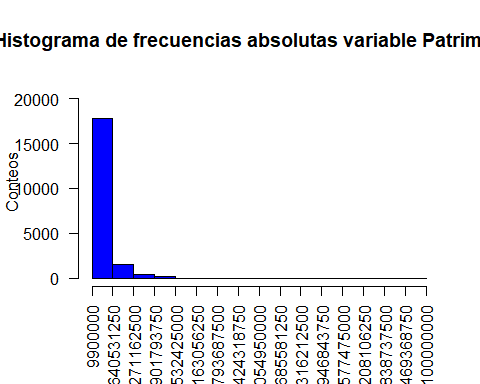
\includegraphics{Ejemplo-Regresión-Múltiple_files/figure-latex/unnamed-chunk-13-1.pdf}

\emph{\textbf{Gráfico residuos estudentizados frente a valores ajustados
por el modelo:}}

\begin{Shaded}
\begin{Highlighting}[]
\KeywordTok{library}\NormalTok{(ggplot2)}
\KeywordTok{ggplot}\NormalTok{(}\DataTypeTok{data =}\NormalTok{ datos, }\KeywordTok{aes}\NormalTok{(}\DataTypeTok{x =} \KeywordTok{predict}\NormalTok{(modelo), }
                        \DataTypeTok{y =} \KeywordTok{abs}\NormalTok{(}\KeywordTok{rstudent}\NormalTok{(modelo))))}\OperatorTok{+}
\StringTok{  }\KeywordTok{geom_hline}\NormalTok{(}\DataTypeTok{yintercept =} \DecValTok{3}\NormalTok{, }\DataTypeTok{color =} \StringTok{"grey"}\NormalTok{, }\DataTypeTok{linetype =} \StringTok{"dashed"}\NormalTok{)}\OperatorTok{+}

\CommentTok{# se identifican en rojo las observaciones con residuos estudentizados}
\KeywordTok{geom_point}\NormalTok{(}\KeywordTok{aes}\NormalTok{(}\DataTypeTok{color =} \KeywordTok{ifelse}\NormalTok{(}\KeywordTok{abs}\NormalTok{(}\KeywordTok{rstudent}\NormalTok{(modelo)) }\OperatorTok{>}\StringTok{ }\DecValTok{2}\NormalTok{, }\StringTok{"red"}\NormalTok{, }\StringTok{"black"}\NormalTok{)))}\OperatorTok{+}
\StringTok{  }\KeywordTok{scale_color_identity}\NormalTok{()}\OperatorTok{+}
\StringTok{  }\KeywordTok{labs}\NormalTok{(}\DataTypeTok{title =} \StringTok{"Distribución de los residuos estudentizados"}\NormalTok{, }
       \DataTypeTok{x =} \StringTok{"Predicción modelo"}\NormalTok{, }
       \DataTypeTok{y =} \StringTok{"Residuos estudentizados"}\NormalTok{)}\OperatorTok{+}
\StringTok{  }\KeywordTok{theme_bw}\NormalTok{() }\OperatorTok{+}\StringTok{ }\KeywordTok{theme}\NormalTok{(}\DataTypeTok{plot.title =} \KeywordTok{element_text}\NormalTok{(}\DataTypeTok{hjust =} \FloatTok{0.5}\NormalTok{))}
\end{Highlighting}
\end{Shaded}

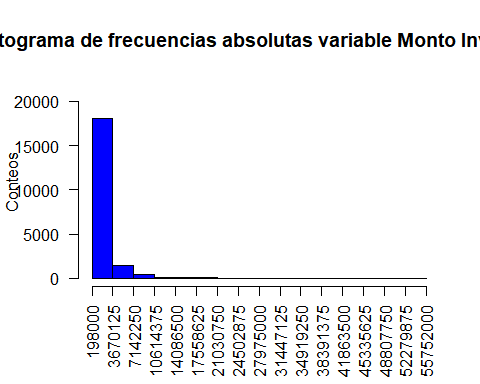
\includegraphics{Ejemplo-Regresión-Múltiple_files/figure-latex/unnamed-chunk-14-1.pdf}

\emph{\textbf{Detección de los residuos estandarizados \textgreater{} 3
considerados como outliers}}

\begin{Shaded}
\begin{Highlighting}[]
\KeywordTok{which}\NormalTok{(}\KeywordTok{rstudent}\NormalTok{(modelo) }\OperatorTok{>}\StringTok{ }\DecValTok{3}\NormalTok{)}
\end{Highlighting}
\end{Shaded}

\begin{verbatim}
## named integer(0)
\end{verbatim}

\begin{Shaded}
\begin{Highlighting}[]
\CommentTok{# Outliers}
\CommentTok{# library(car) # En R_3.5}
\CommentTok{# outlierTest(modelo)}

\CommentTok{# install.packages("outliers")}
\KeywordTok{library}\NormalTok{(outliers)}
\end{Highlighting}
\end{Shaded}

\begin{verbatim}
## 
## Attaching package: 'outliers'
\end{verbatim}

\begin{verbatim}
## The following object is masked from 'package:psych':
## 
##     outlier
\end{verbatim}

\begin{Shaded}
\begin{Highlighting}[]
\NormalTok{test <-}\StringTok{ }\KeywordTok{grubbs.test}\NormalTok{(modelo}\OperatorTok{$}\NormalTok{residuals )}
\NormalTok{test}
\end{Highlighting}
\end{Shaded}

\begin{verbatim}
## 
##  Grubbs test for one outlier
## 
## data:  modelo$residuals
## G.Maine = 2.19810, U = 0.89938, p-value = 0.6199
## alternative hypothesis: lowest value -1.47514185671001 is an outlier
\end{verbatim}

La prueba de Grubbs permite detectar si el valor más alto o más bajo en
un conjunto de datos es un valor atípico.

La prueba de Grubbs detecta un valor atípico a la vez (valor más alto o
más bajo), por lo que las hipótesis nula y alternativa son las
siguientes:

\begin{verbatim}
H0: el valor más alto no es un valor atípico
H1: el valor más alto es un valor atípico
\end{verbatim}

si queremos probar el valor más alto, o:

\begin{verbatim}
H0: el valor más bajo no es un valor atípico
H1: el valor más bajo es un valor atípico  
\end{verbatim}

si queremos probar el valor más bajo.

Como para cualquier prueba estadística, si el valor p es menor que el
umbral de significancia elegido (generalmente α = 0.05), entonces se
rechaza la hipótesis nula y concluiremos que el valor más bajo / más
alto es un valor atípico. Por el contrario, si el valor p es mayor o
igual que el nivel de significancia, no se rechaza la hipótesis nula, y
concluiremos que, con base en los datos, no rechazamos la hipótesis de
que el valor más bajo / más alto no es un valor atípico.

Tenga en cuenta que la prueba de Grubbs no es apropiada para un tamaño
de muestra de 6 o menos (n≤6).

\emph{\textbf{COLINEALIDAD - FACTOR DE INFLACIÓN DE LA VARIANZA:}}

\emph{\textbf{VIF=1/(1-R\^{}2) donde R\^{}2 es el coeficiente de
determinación de la regresión del j-ésimo regresor sobre el resto. El
valor mínimo de VIF es 1 y un VIF\textgreater{}10 puede indicar la
existencia colinealidad (o \textgreater{}5 siend estricto\ldots{}) }}

\begin{Shaded}
\begin{Highlighting}[]
\KeywordTok{library}\NormalTok{(caret)}
\KeywordTok{library}\NormalTok{(MASS)}
\KeywordTok{library}\NormalTok{(tidyverse)}
\NormalTok{car}\OperatorTok{::}\KeywordTok{vif}\NormalTok{(modelo)}
\end{Highlighting}
\end{Shaded}

\begin{verbatim}
##    habitantes      ingresos analfabetismo        muerte     graduados 
##      1.634268      3.275340      5.475516      3.028169      3.229221 
##       heladas          area densidad_pobl 
##      2.501893      2.429078      2.377250
\end{verbatim}

\emph{\textbf{Autocorrelación: Estadístico Durbyn Whatson:}}

\begin{Shaded}
\begin{Highlighting}[]
\CommentTok{# graficamos el nuestros valores estimados}
\KeywordTok{plot}\NormalTok{(datos}\OperatorTok{$}\NormalTok{esp_vida, }\KeywordTok{fitted}\NormalTok{(modelo), }\DataTypeTok{cex =} \DecValTok{1}\NormalTok{, }\DataTypeTok{pch =} \DecValTok{21}\NormalTok{, }\DataTypeTok{bg =} \StringTok{"darkorange"}\NormalTok{, }\DataTypeTok{col =} \StringTok{"black"}\NormalTok{)}
\KeywordTok{lines}\NormalTok{(}\KeywordTok{fitted}\NormalTok{(modelo))}
\end{Highlighting}
\end{Shaded}

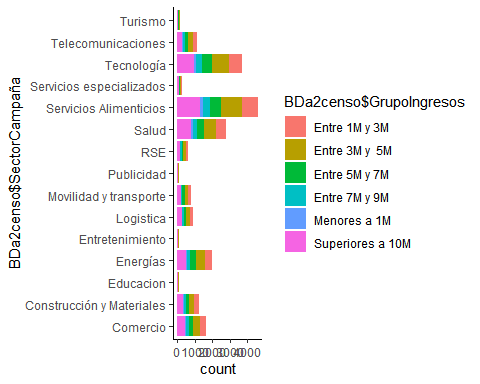
\includegraphics{Ejemplo-Regresión-Múltiple_files/figure-latex/unnamed-chunk-17-1.pdf}

\emph{\textbf{Test de validación de autocorrelación, a través del
estadístico de Durbyn \& Whatson}}

\emph{\textbf{Las Hipótesis en juego son:}}

\emph{\textbf{Ho: La autocorrelación verdadera es igual a 0}}
\emph{\textbf{Ha: La autocorrelación verdadera es mayor que 0}}

\emph{\textbf{En este caso se desea NO RECHAZAR LA HIPOTESIS NULA}}

\begin{Shaded}
\begin{Highlighting}[]
\CommentTok{# Cargamos el paquete lmtest para realizar la prueba Durbin-Watson}
\KeywordTok{library}\NormalTok{(lmtest) }
\end{Highlighting}
\end{Shaded}

\begin{verbatim}
## Loading required package: zoo
\end{verbatim}

\begin{verbatim}
## 
## Attaching package: 'zoo'
\end{verbatim}

\begin{verbatim}
## The following objects are masked from 'package:base':
## 
##     as.Date, as.Date.numeric
\end{verbatim}

\begin{Shaded}
\begin{Highlighting}[]
\KeywordTok{dwtest}\NormalTok{(modelo)}
\end{Highlighting}
\end{Shaded}

\begin{verbatim}
## 
##  Durbin-Watson test
## 
## data:  modelo
## DW = 1.9653, p-value = 0.4526
## alternative hypothesis: true autocorrelation is greater than 0
\end{verbatim}

\emph{\textbf{UN PEQUEÑO EJEMPLO DE UN AJUSTE DE REGRESIÓN 3D (Dos
variables idependientes X's que expliquen a Y):}}

\begin{Shaded}
\begin{Highlighting}[]
\KeywordTok{library}\NormalTok{(rgl)}

\NormalTok{modelo2 <-}\StringTok{ }\KeywordTok{lm}\NormalTok{(esp_vida }\OperatorTok{~}\StringTok{ }\NormalTok{muerte }\OperatorTok{+}\StringTok{ }\NormalTok{graduados, }\DataTypeTok{data=}\NormalTok{datos)}

\CommentTok{# predicción del modelo2}
\KeywordTok{summary}\NormalTok{(modelo2)}
\end{Highlighting}
\end{Shaded}

\begin{verbatim}
## 
## Call:
## lm(formula = esp_vida ~ muerte + graduados, data = datos)
## 
## Residuals:
##      Min       1Q   Median       3Q      Max 
## -1.66758 -0.41801  0.05602  0.55913  2.05625 
## 
## Coefficients:
##             Estimate Std. Error t value Pr(>|t|)    
## (Intercept) 70.29708    1.01567  69.213  < 2e-16 ***
## muerte      -0.23709    0.03529  -6.719 2.18e-08 ***
## graduados    0.04389    0.01613   2.721  0.00909 ** 
## ---
## Signif. codes:  0 '***' 0.001 '**' 0.01 '*' 0.05 '.' 0.1 ' ' 1
## 
## Residual standard error: 0.7959 on 47 degrees of freedom
## Multiple R-squared:  0.6628, Adjusted R-squared:  0.6485 
## F-statistic:  46.2 on 2 and 47 DF,  p-value: 8.016e-12
\end{verbatim}

\begin{Shaded}
\begin{Highlighting}[]
\CommentTok{# Haciendo la Grilla}
\NormalTok{plotdata2 <-}\StringTok{ }\KeywordTok{expand.grid}\NormalTok{(}\DataTypeTok{graduados=}\KeywordTok{seq}\NormalTok{(}\DecValTok{34}\NormalTok{,}\DecValTok{70}\NormalTok{,}\DataTypeTok{by=}\DecValTok{2}\NormalTok{),}\DataTypeTok{muerte=}\KeywordTok{seq}\NormalTok{(}\DecValTok{1}\NormalTok{,}\DecValTok{16}\NormalTok{,}\DataTypeTok{by=}\DecValTok{1}\NormalTok{))}
\NormalTok{plotdata2}\OperatorTok{$}\NormalTok{pred1 <-}\StringTok{ }\KeywordTok{predict}\NormalTok{(modelo2,}\DataTypeTok{newdata=}\NormalTok{plotdata2)}


\CommentTok{# Graficando la Regresión Múltiple en 3D}
\KeywordTok{with}\NormalTok{(datos,}\KeywordTok{plot3d}\NormalTok{(graduados, muerte, esp_vida,  }\DataTypeTok{col=}\StringTok{"blue"}\NormalTok{, }\DataTypeTok{size=}\DecValTok{1}\NormalTok{, }\DataTypeTok{type=}\StringTok{"s"}\NormalTok{))}
\KeywordTok{with}\NormalTok{(plotdata2,}\KeywordTok{surface3d}\NormalTok{(}\KeywordTok{unique}\NormalTok{(graduados),}\KeywordTok{unique}\NormalTok{(muerte),pred1,}
                       \DataTypeTok{alpha=}\FloatTok{0.5}\NormalTok{,}\DataTypeTok{front=}\StringTok{"line"}\NormalTok{, }\DataTypeTok{back=}\StringTok{"line"}\NormalTok{))}
\end{Highlighting}
\end{Shaded}

\subsubsection{Algorítmo automático de
selección}\label{algoruxedtmo-automuxe1tico-de-selecciuxf3n}

\emph{\textbf{Este algorítimo automático identifica cuál es la mejor
combinación de variables independeintes X's que proporcionan el R\^{}2
más grande (Selección de los mejores predictores).}}

En este caso se van a emplear la estrategia de stepwise mixto.\\
El estadístico empleado para determinar la calidad del modelo va a ser
Akaike(AIC). En este sentido, el modelo con el menor AIC será el mejor
modelo:

\begin{Shaded}
\begin{Highlighting}[]
\KeywordTok{step}\NormalTok{(}\DataTypeTok{object =}\NormalTok{ modelo, }\DataTypeTok{direction =} \StringTok{"both"}\NormalTok{, }\DataTypeTok{trace =} \DecValTok{1}\NormalTok{)}
\end{Highlighting}
\end{Shaded}

\begin{verbatim}
## Start:  AIC=-22.89
## esp_vida ~ habitantes + ingresos + analfabetismo + muerte + graduados + 
##     heladas + area + densidad_pobl
## 
##                 Df Sum of Sq    RSS     AIC
## - analfabetismo  1    0.3050 22.373 -24.208
## - area           1    0.3564 22.425 -24.093
## - ingresos       1    0.4120 22.480 -23.969
## <none>                       22.068 -22.894
## - heladas        1    1.1102 23.178 -22.440
## - densidad_pobl  1    1.2288 23.297 -22.185
## - graduados      1    1.8225 23.891 -20.926
## - habitantes     1    2.5095 24.578 -19.509
## - muerte         1   23.8173 45.886  11.707
## 
## Step:  AIC=-24.21
## esp_vida ~ habitantes + ingresos + muerte + graduados + heladas + 
##     area + densidad_pobl
## 
##                 Df Sum of Sq    RSS     AIC
## - area           1    0.1427 22.516 -25.890
## - ingresos       1    0.2316 22.605 -25.693
## <none>                       22.373 -24.208
## - densidad_pobl  1    0.9286 23.302 -24.174
## - graduados      1    1.5218 23.895 -22.918
## + analfabetismo  1    0.3050 22.068 -22.894
## - habitantes     1    2.2047 24.578 -21.509
## - heladas        1    3.1324 25.506 -19.656
## - muerte         1   26.7071 49.080  13.072
## 
## Step:  AIC=-25.89
## esp_vida ~ habitantes + ingresos + muerte + graduados + heladas + 
##     densidad_pobl
## 
##                 Df Sum of Sq    RSS     AIC
## - ingresos       1     0.132 22.648 -27.598
## - densidad_pobl  1     0.786 23.302 -26.174
## <none>                       22.516 -25.890
## - graduados      1     1.424 23.940 -24.824
## + area           1     0.143 22.373 -24.208
## + analfabetismo  1     0.091 22.425 -24.093
## - habitantes     1     2.332 24.848 -22.962
## - heladas        1     3.304 25.820 -21.043
## - muerte         1    32.779 55.295  17.033
## 
## Step:  AIC=-27.6
## esp_vida ~ habitantes + muerte + graduados + heladas + densidad_pobl
## 
##                 Df Sum of Sq    RSS     AIC
## - densidad_pobl  1     0.660 23.308 -28.161
## <none>                       22.648 -27.598
## + ingresos       1     0.132 22.516 -25.890
## + analfabetismo  1     0.061 22.587 -25.732
## + area           1     0.043 22.605 -25.693
## - habitantes     1     2.659 25.307 -24.046
## - heladas        1     3.179 25.827 -23.030
## - graduados      1     3.966 26.614 -21.529
## - muerte         1    33.626 56.274  15.910
## 
## Step:  AIC=-28.16
## esp_vida ~ habitantes + muerte + graduados + heladas
## 
##                 Df Sum of Sq    RSS     AIC
## <none>                       23.308 -28.161
## + densidad_pobl  1     0.660 22.648 -27.598
## + ingresos       1     0.006 23.302 -26.174
## + analfabetismo  1     0.004 23.304 -26.170
## + area           1     0.001 23.307 -26.163
## - habitantes     1     2.064 25.372 -25.920
## - heladas        1     3.122 26.430 -23.877
## - graduados      1     5.112 28.420 -20.246
## - muerte         1    34.816 58.124  15.528
\end{verbatim}

\begin{verbatim}
## 
## Call:
## lm(formula = esp_vida ~ habitantes + muerte + graduados + heladas, 
##     data = datos)
## 
## Coefficients:
## (Intercept)   habitantes       muerte    graduados      heladas  
##   7.103e+01    5.014e-05   -3.001e-01    4.658e-02   -5.943e-03
\end{verbatim}

\emph{\textbf{Elección del Modelo Final}} En Conclusión: El mejor modelo
resultante del proceso de selección ha sido:

\begin{Shaded}
\begin{Highlighting}[]
\NormalTok{modelo <-}\StringTok{ }\NormalTok{(}\KeywordTok{lm}\NormalTok{(}\DataTypeTok{formula =}\NormalTok{ esp_vida }\OperatorTok{~}\StringTok{ }\NormalTok{habitantes }\OperatorTok{+}\StringTok{ }\NormalTok{muerte }\OperatorTok{+}\StringTok{ }\NormalTok{graduados }\OperatorTok{+}
\StringTok{                }\NormalTok{heladas, }\DataTypeTok{data =}\NormalTok{ datos))}

\KeywordTok{summary}\NormalTok{(modelo)}
\end{Highlighting}
\end{Shaded}

\begin{verbatim}
## 
## Call:
## lm(formula = esp_vida ~ habitantes + muerte + graduados + heladas, 
##     data = datos)
## 
## Residuals:
##      Min       1Q   Median       3Q      Max 
## -1.47095 -0.53464 -0.03701  0.57621  1.50683 
## 
## Coefficients:
##               Estimate Std. Error t value Pr(>|t|)    
## (Intercept)  7.103e+01  9.529e-01  74.542  < 2e-16 ***
## habitantes   5.014e-05  2.512e-05   1.996  0.05201 .  
## muerte      -3.001e-01  3.661e-02  -8.199 1.77e-10 ***
## graduados    4.658e-02  1.483e-02   3.142  0.00297 ** 
## heladas     -5.943e-03  2.421e-03  -2.455  0.01802 *  
## ---
## Signif. codes:  0 '***' 0.001 '**' 0.01 '*' 0.05 '.' 0.1 ' ' 1
## 
## Residual standard error: 0.7197 on 45 degrees of freedom
## Multiple R-squared:  0.736,  Adjusted R-squared:  0.7126 
## F-statistic: 31.37 on 4 and 45 DF,  p-value: 1.696e-12
\end{verbatim}

\end{document}
